%!TEX root = ../thesis_a4.tex

\chapter[A scheme for folksonomy-based tag recommendation][A scheme for folksonomy-based tag rec.]{A scheme for folksonomy-based tag recommendation}
\label{sec:general}

\section{Introduction}
\label{sec:general:introduction}

%Collaborative tagging has emerged as a common and successful solution for labelling and organising huge amounts of digital content, being adopted by many well-known sites such as Youtube, Flickr, Last.fm, or Delicious~\cite{marlow2006}. In collaborative tagging, users assign a number of free-form semantically-meaningful textual labels (tags) to information resources. These tags can be then used for many purposes, including retrieval, browsing and categorisation~\cite{Bischoff2008}. For instance, they can be used for matching user queries with resources tags, or for building tag clouds to navigate across resources. Such usages are of special importance for platforms that share multimedia content such as videos, images, or audio, since such contents can not be so directly and straightforwardly indexed as it would be done with textual data like books or web pages~\cite{Bischoff2008}. Because of this importance, collaborative tagging systems have been widely researched in the last few years. 
%In particular, a focus has been given to collaborative tagging dynamics and user behaviour \cite{marlow2006,halpin2006,golder2006,farooq2007} and to automatic tag classification methods based on user motivations~\cite{Bischoff2008,cantador2010}.

%Nevertheless, collaborative tagging systems suffer from a number of well-known issues~\cite{halpin2006,cantador2010}, which include tag scarcity, the use of different labels to refer to a single concept (synonymy), the ambiguity in the meaning of certain labels (polysemy), the commonness of typographical errors, the use of user-specific naming conventions, or even the use of different languages. One strategy for trying to overcome these problems, and thus to obtain more comprehensive and consistent tag assignments, is the use of tag recommendation systems to help users in the tagging process~\cite{jaske2007}. In that case, when users are labeling online resources, tag recommendation systems automatically suggest new tags that can also be meaningful or relevant for the resource being described. This way, tag recommendation serves the purpose of consolidating the tag vocabulary among users in a collaborative tagging system~\cite{jaske2007}. In addition, tag recommendation systems can be used, in an off-line mode, to extend the descriptions of information resources by automatically adding new tags.

In this chapter we describe a general scheme for tag recommendation in large-scale tagging systems. The approach we describe here is based on tag co-occurrence in folksonomies, meaning that we do not perform any content analysis of the information resources for which we produce tag recommendations. We uniquely rely on the tag co-occurrence information that can be derived from the folksonomy itself.
As the scheme we describe only relies on this information, it is rather domain-independent and could be easily adapted to other tagging systems, either alone or as a complement of perhaps more specific content-based strategies. 
Hence, our approach is highly related to those outlined in Sec.~\ref{sec:soa:tag_recommendation_folkosnomy_analysis} and, in particular, to the tag recommendation methods described by~\cite{Sigurbjornsson2008} and~\cite{Garg2008}. 
%Tag recommendation systems based on this approach have been proposed for the image~\citep{Anderson2008,Sigurbjornsson2008,Garg2008,Wu2009,Liu2010a,Rae2010}, video~\citep{Ballan2010}, and bookmark domains~\citep{Lipczak2008,Song2008,Cao2009,meo2009,Zhang2009}.

A particularly interesting aspect of our tag recommendation scheme, which differentiates it from previous works, is a step focused on automatically selecting the number of tags to recommend. That step is accomplished by considering the relative relevance scores of a set of candidate tags with respect to a set of input tags (see below). Other tag recommendation methods generally do not consider this aspect and evaluate their solutions at different numbers of $\nRecommendedTagsInEvaluation$ recommended tags (Sec.~\ref{sec:soa:tag_recommendation_folkosnomy_analysis}). 
This is an unrealistic situation as, in a real-world scenario, only a limited number of tags can be suggested to users, and an arbitrary decision of this number may yield suboptimal recommendations either missing relevant tags or suggesting too many non-relevant ones.
%We believe that a tag recommendation method such as the one we propose here can be useful to obtain more comprehensive and coherent descriptions of tagged resources, and help the emergence of less noisy and more consistent folksonomies. This can greatly benefit organisation, browsing and reuse of online content, and also leverage the value of folksonomies as reliable sources for knowledge-mining~\cite{al2007exploring, limpens2009linking}. 

We propose eight tag recommendation methods which are based on the aforementioned general scheme. The proposed methods, jointly with several baselines, are evaluated with data coming from Freesound and Flickr. For the best scoring methods, we also analyse the influence of their configurable parameters. Overall, we perform more than 100 different experiments and compute around seven million tag recommendations. 

The rest of this chapter is organized as follows. 
In Sec.~\ref{sec:general:method} we describe the different steps of our tag recommendation scheme and the strategies we propose to compute each step.
Then, in Sec.~\ref{sec:general:evaluation_methodology}, we outline the characteristics of the evaluation datasets and describe the methodology we followed to evaluate our methods and the considered baselines.
The results of our evaluation are reported in Sec.~\ref{sec:general:results}, and the chapter ends with a discussion about our findings and future work (Sec.~\ref{general:sec:discussion}). 


\section{Method}
\label{sec:general:method}

\begin{figure}[t]
  \centerline{
  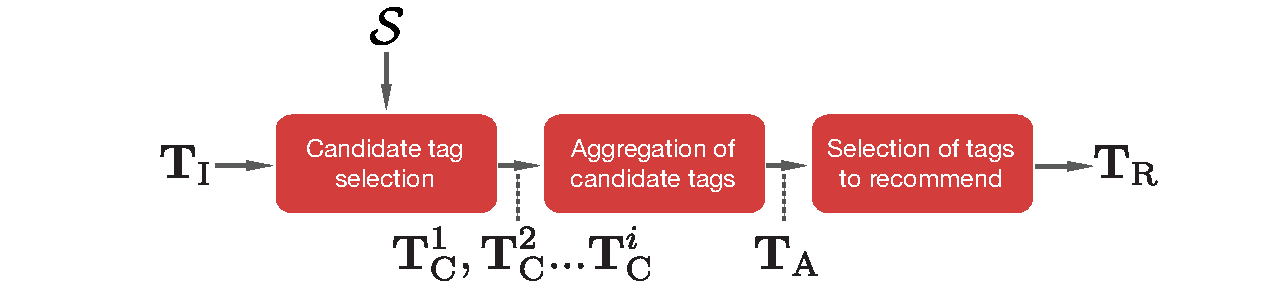
\includegraphics[width=\figSizeMax]{ch03_general/pics/00_diagram_alt.pdf}}
  \caption[Block diagram of the tag recommendation scheme]{Block diagram of the described tag recommendation scheme.}
  \label{general:fig:diagram}
\end{figure}

Given a set of input tags $\inputTags$ and a tag-tag similarity matrix $\similarityMatrix$ derived from a folksonomy $\folksonomy$, the general scheme for tag recommendation outputs a set of recommended tags $\recommendedTags$ (Fig.~\ref{general:fig:diagram}). 
%The folksonomy can be defined as a set of tag assignments $\folksonomy \subseteq \users \times \tags \times \resources$, where $\users$, $\tags$, and $\resources$ denote sets of users, tags, and resources, respectively~\cite{Mika2007a}\footnote{Mika~\citeyear{Mika2007a} uses the terminology Actor, Concept, and Instance ($A$, $C$ and $I$) to denote what we call User, Tag, and Resource ($\users$, $\tags$ and $\resources$). We adopted the latter terminology as it more closely relates with the data we are dealing with.}. 
The described scheme is composed of three independent steps: 1) Candidate tag selection, 2) Aggregation of candidate tags, and 3) Selection of tags to recommend. For Step 1, we propose three variants based on different similarity measures widely used in the literature~\citep[tag co-occurrence, cosine and Jaccard similarity;][]{halpin2006,jaske2007,Mika2007a,Sigurbjornsson2008,meo2009,Markines2009}. For Step 2, we propose two aggregation strategies (Similarity-based and Rank-based). For Step 3, we propose four selection strategies (Percentage, Statistical Test, Kernel Percentage and Linear Regression). What follows is a brief overview of these steps. In-depth descriptions are given in subsequent sections.

\begin{itemize}
  \item Step 1: Candidate tag selection. Given $\inputTags$ and a tag-tag similarity matrix $\similarityMatrix$ derived from $\folksonomy$, this step retrieves a set of $\nCandidateTagsPerInputTag$ candidate tags $\candidateTagsPerInputTag$ for each input tag $\inputTag$. %The retrieval of these candidates is based on tag-tag semantic similarity measures derived from $\folksonomy$.

  \item Step 2: Aggregation of candidate tags. This step takes the sets of candidates $\candidateTagsPerInputTag$, assigns a score value to each individual tag, and aggregates all candidates to form a single list of tags with assigned scores $\aggregatedCandidateTags$.

  \item Step 3: Selection of tags to recommend. This step automatically selects which tags to recommend given the candidate tags and score values of $\aggregatedCandidateTags$. The output of this step is the final set of recommended tags $\recommendedTags$.
\end{itemize}


\subsection{Candidate tag selection}
\label{sec:general:step1}

%Mika's model considers three finite sets of objects $\mathbf{A}$, $\mathbf{C}$ and $\mathbf{I}$ which correspond to ``actors'' (i.e.,~users), ``concepts'' (i.e.,~tags) and ``instances'' (i.e.,~resources). In this thesis, instead of the variables $\mathbf{A}$, $\mathbf{C}$ and $\mathbf{I}$ defined by ~\cite{Mika2007a}, we employ the notation $\users$, $\tags$ and $\resources$ respectively, which more closely relates to the ``users'', ``tags'' and ``resources'' terminology that we use.
%The sets of users, tags and resources are represented as nodes in the graph such that nodes $\vertices=\users\cup \tags\cup \resources$. The ternary relations between a user, a tag and a resource (i.e.,~tag applications) are then represented as the edges of the graph $\edges=\{\{\user,\tag,\resource\}| (\user,\tag,\resource)$ $\in \folksonomy\}$. Hence, the graph $\graph$ that represents a folksonomy $\folksonomy$ is finally defined as $\graph(\folksonomy)=\left\langle \vertices,\edges \right\rangle$. 
%The tripartite graph can be unfolded into a bipartite graph after discarding one of the three sets of nodes (i.e.,~$\users$, $\tags$ or $\resources$). In this way, it is possible to obtain the graph $\bipartiteGraphTagsUsers$ which relates tags and users, the graph $\bipartiteGraphUsersResources$ which relates users and resources, and the graph $\bipartiteGraphTagsResources$ which relates tags and resources. That last bipartite graph is the view of the folksonomy that we work with in this thesis, as it allows to derive relations between tags on the basis of their shared resources and vice versa.

We start the recommendation process by obtaining a number of related candidate tags to the set of input tags $\inputTags$. 
For each input tag $\inputTag$, we get a set of candidates $\candidateTagsPerInputTag$ by selecting the $\nCandidateTagsPerInputTag$ closest tags to $\inputTag$ according to a tag-tag similarity measure. For this purpose, we build a tag-tag similarity matrix $\similarityMatrix$ based on the tag assignment information contained in the folksonomy $\folksonomy$. Note that $\similarityMatrix$ is not dependent of the particular $\inputTag$ for which we are selecting candidates. Therefore, it only needs to be computed once for a given~$\folksonomy$\footnote{As is described later in Sec.~\ref{sec:general:datasets}, we filter out the least frequent tags of our folksonomy in order to reduce the computational complexity of $\similarityMatrix$.}. 

To represent the folksonomy $\folksonomy$, we use the model proposed by~\cite{Mika2007a}. Mika's model considers three finite sets of objects $\mathbf{A}$, $\mathbf{C}$ and $\mathbf{I}$, which correspond to ``actors'' (i.e.,~users), ``concepts'' (i.e.,~tags) and ``instances'' (i.e.,~resources), respectively. In this thesis, instead of the variables $\mathbf{A}$, $\mathbf{C}$ and $\mathbf{I}$ defined by ~\cite{Mika2007a}, we employ the notation $\users$, $\tags$ and $\resources$, which more closely relates to the ``users'', ``tags'' and ``resources'' terminology that we use.
The sets of users, tags and resources are represented as nodes in the graph such that the set of nodes $\vertices$ is defined as $\vertices=\users\cup \tags\cup \resources$. The ternary relations between a user, a tag and a resource (i.e.,~tag applications) are then represented as the edges of the graph $\edges=\{\{\user,\tag,\resource\}| (\user,\tag,\resource)$ $\in \folksonomy\}$. Hence, the graph $\graph$ that represents a folksonomy $\folksonomy$ is finally defined as $\graph(\folksonomy)=\left\langle \vertices,\edges \right\rangle$. 
%As we described in the previous chapter, Sec.~\ref{sec:soa:tag_recommendation_folkosnomy_analysis}, a folksonomy $\folksonomy$ can be naturally modelled as a tripartite hypergraph $\graph(\folksonomy)=\left\langle \vertices,\edges \right\rangle$, where vertices are given by three finite sets of objects, $\vertices=\users\cup \tags\cup \resources$, and each edge $\edges$ represents a tag-resource association performed by a user, $\edges=\{\{\user,\tag,\resource\}| (\user,\tag,\resource)$ $\in \folksonomy\}$ \citep{Mika2007a}. 

We unfold $\graph(\folksonomy)$ into the bipartite graph $\bipartiteGraphTagsResources$, which only reflects the associations between tags and resources. 
The bipartite graph $\bipartiteGraphTagsResources$ can be represented as a matrix $\associationMatrix = \left\{ \associationMatrixElement_{i,j} \right\}$, where $\associationMatrixElement_{i,j} = 1$ if tag $\tag_i$ has been used to label resource $\resource_j$, and $\associationMatrixElement_{i,j} = 0$ otherwise. 
We then define the matrix $\similarityMatrix$ so that
\begin{equation}
  \similarityMatrix = \associationMatrixMultiplication',
  \label{general:eq:Sim}
\end{equation}
which corresponds to a one-mode network connecting tags on the basis of shared resources~\citep{Mika2007a}. The symbol $'$ denotes matrix transposition. Elements $\similarityMatrixElement_{i,j}$ of $\similarityMatrix$ indicate the number of resources in which tags $\tag_i$ and $\tag_j$ appear together. Therefore, the diagonal of $\similarityMatrix$ represents the total number of different resources labelled with a tag $\tag_{i=j}$.

At this point, $\similarityMatrix$ can be interpreted as a tag-tag similarity matrix based on absolute co-occurrence. That is to say, the similarity between tags $\tag_i$ and $\tag_j$ is represented by the total number of times they appear together. This is the first similarity measure we use for our tag recommendation method. In order to obtain the rest of the aforementioned similarity measures, we apply different normalisation procedures to $\similarityMatrix$. Cosine similarity is defined as
\begin{equation}
  \similarityMatrixElement_{\tagb_i,\tagb_j} = \frac{\sum_{n} \associationMatrixElement_{i,n} \associationMatrixElement_{j,n} }{ \sqrt{\sum_{n} {\associationMatrixElement_{i,n}}^2} \sqrt{\sum_{n} {\associationMatrixElement_{j,n}}^2} } .
  \label{general:eq:CosineSim}
\end{equation}
Given that rows $\associationMatrixRow_i$ and $\associationMatrixRow_j$ are bit vectors (the only possible values are $0$ or $1$), $\sum_{n}{\associationMatrixElement_{i,n} \associationMatrixElement_{j,n}}$ is equivalent to the absolute co-occurrence between tags $\tag_i$ and $\tag_j$, while $\sum_{n}{\associationMatrixElement_{i,n}}^2$ and $\sum_{n}{\associationMatrixElement_{j,n}}^2$ is equivalent to the total number of occurrences of tags $\tag_i$ and $\tag_j$, respectively (the total number of resources labeled with $\tag_i$ and $\tag_j$). Therefore, cosine similarity can be obtained by dividing each element in $\similarityMatrix$ (Eq.~\ref{general:eq:Sim}) by $\sqrt{\similarityMatrixElement_{\tag_i,\tag_i} }\sqrt{\similarityMatrixElement_{\tag_j,\tag_j} }$. Similarly, the Jaccard index is defined as
\begin{equation}
  \similarityMatrixElement_{\tagb_i,\tagb_j} = \frac{\sum_{n} \associationMatrixElement_{i,n} \associationMatrixElement_{j,n} }{ \sum_{n} {\associationMatrixElement_{i,n}}^2 + \sum_{n} {\associationMatrixElement_{j,n}}^2 -  \sum_{n} \associationMatrixElement_{i,n} \associationMatrixElement_{j,n} } ,
  \label{general:eq:JacIndex}
\end{equation}
which is equivalent to dividing each element in $\similarityMatrix$ by $\similarityMatrixElement_{\tag_i,\tag_i} + \similarityMatrixElement_{\tag_j,\tag_j} - \similarityMatrixElement_{\tag_i,\tag_j}$. Independently of the similarity measure, $\similarityMatrix$ can be represented as a graph where nodes correspond to tags and edges represent the similarities between two tags (Fig.~\ref{general:fig:graph}).

Once we have a tag similarity matrix $\similarityMatrix$, we iterate over the input tags $\inputTags$ and get, for each element $\inputTag$, a set of candidates $\candidateTagsPerInputTag$. Specifically, we select the $\nCandidateTagsPerInputTag$ most similar tags to $\inputTag$ (i.e.,~the $\nCandidateTagsPerInputTag$ most similar graph neighbours of $\inputTag$) and keep these similarity values for further processing. Hence, for instance, if our method is fed with three input tags, it will get a maximum of $3\nCandidateTagsPerInputTag$ candidate tags (separated into three sets), provided that all three input tags have at least $\nCandidateTagsPerInputTag$ graph neighbours.

\begin{figure}
  \centerline{
  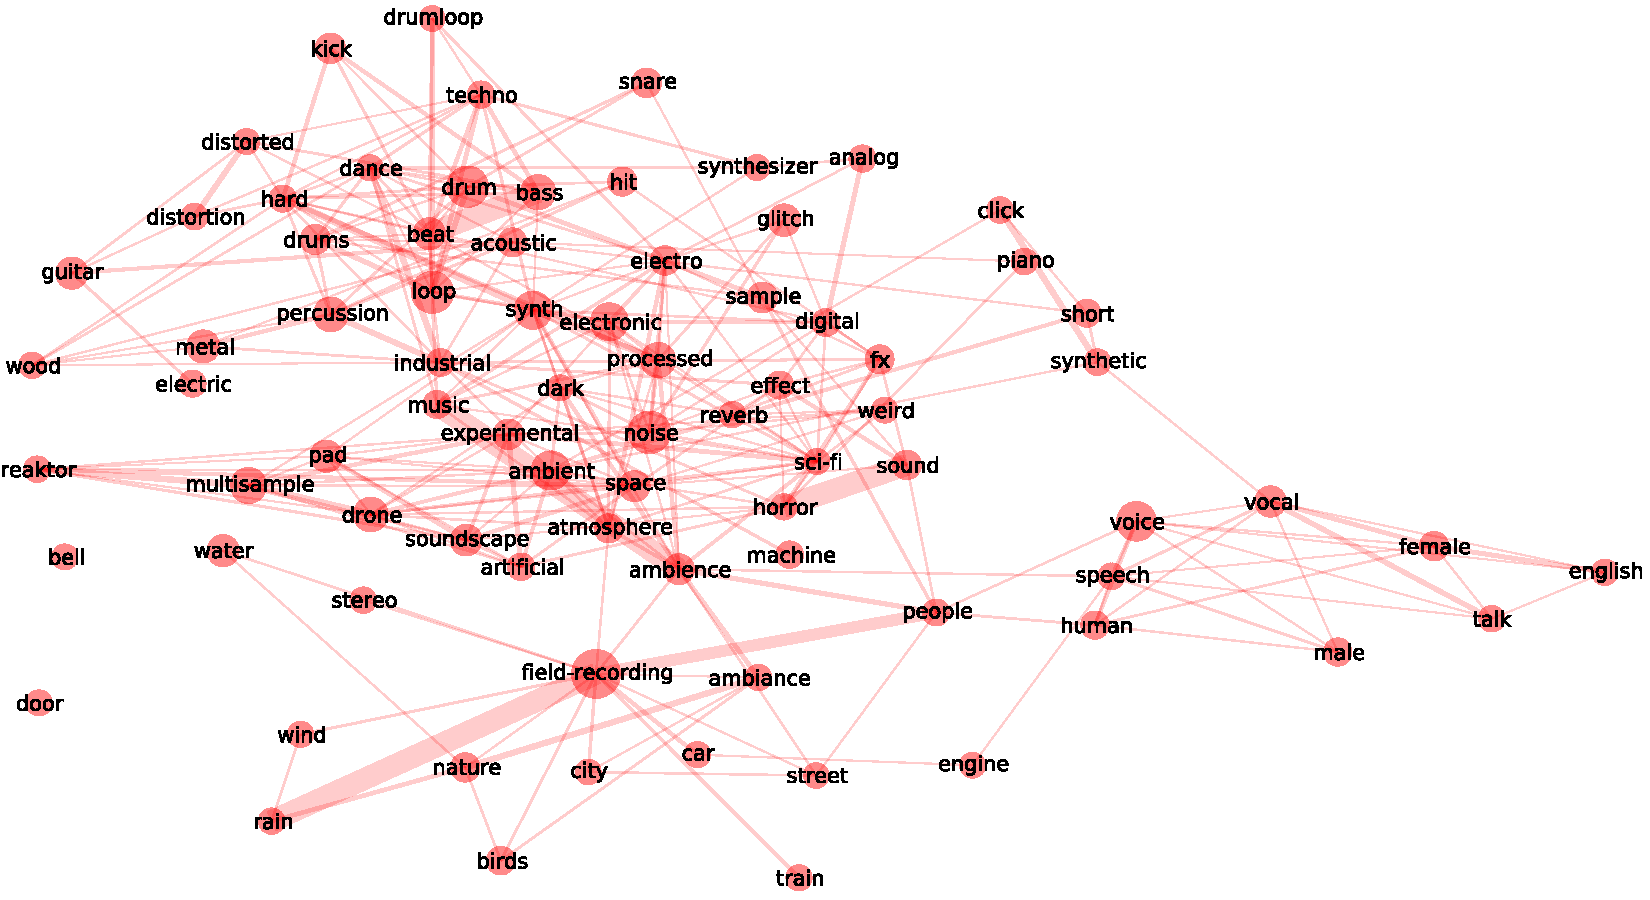
\includegraphics[width=\figSizeMax]{ch03_general/pics/01_graph_visualisation.pdf}}
  \caption[Graph visualisation of a tag-tag similarity matrix $\similarityMatrix$]{Graph visualisation of a tag-tag similarity matrix $\similarityMatrix$ built using cosine similarity and a subset of the Freesound folksonomy. Edge widths represent the cosine similarity between two tags. Tag size is a logarithmic function of the absolute tag frequency. For visualisation purposes, only edges above a certain degree of similarity and tags above a certain level of absolute frequency are shown.
  }
  \label{general:fig:graph}
\end{figure}


\subsection{Aggregation of candidate tags}
\label{sec:gen:step_2_aggregation}

The next step of our tag recommendation scheme takes all the sets of candidates $\candidateTagsPerInputTag$, assigns a score value $\scoreCandidateTag_j$ to every candidate $\candidateTag$ in $\candidateTagsPerInputTag$, and then aggregates all sets into a single list of tags with assigned scores $\aggregatedCandidateTags$. The output of this step, $\aggregatedCandidateTags$, is a list of tuples where each element contains a tag and an assigned score. To accomplish this step, we propose two different strategies:


\subsubsection{Similarity-based Strategy}

In the Similarity-based Strategy, the $j$-th candidate tag $\candidateTag$ of $\candidateTagsPerInputTag$ is assigned a score $\scoreCandidateTag_j$ that directly corresponds to the similarity value between the candidate tag and the corresponding input tag $\inputTag$, i.e.,~$\scoreCandidateTag_j = \similarityMatrixElement_{x,y}$, where $x=\candidateTag$ and $y=\inputTag$. After that, the list of tuples $\aggregatedCandidateTags$ is constructed as the union of all sets of candidates $\candidateTagsPerInputTag$ and their scores. 
If a particular tag has duplicates in $\aggregatedCandidateTags$ (which can happen if a given tag appears in several sets of candidates $\candidateTagsPerInputTag$), we only keep one occurrence and set its score to the sum of all the scores of the duplicates of that tag. This way we promote tags that are considered to be similar to more than one input tag. Moreover, as we do not want to recommend tags that are already part of $\inputTags$, we remove any occurrences of these tags in $\aggregatedCandidateTags$. 
We finally normalise the assigned scores by dividing them by the number of input tags $|\inputTags|$. 

\subsubsection{Rank-based Strategy}

The Rank-based Strategy only differs from the Similarity-based Strategy above in the way scores are assigned. Instead of directly using the similarity values from Step 1, we assign discrete ranks. For this purpose, we sort each set $\candidateTagsPerInputTag$ by similarity values in descending order, and assign scores as
$\scoreCandidateTag_j = \nCandidateTagsPerInputTag - (\positionOfCandidateTagInList -1)$, 
where $\positionOfCandidateTagInList$ is the position of the $j$-th tag in $\candidateTagsPerInputTag$ after sorting (thus $\positionOfCandidateTagInList$ ranges from 1 to $\nCandidateTagsPerInputTag$). Notice that the most similar tag to every input tag will be assigned a score of $\nCandidateTagsPerInputTag$. Even if a particular set $\candidateTagsPerInputTag$ contains less than $\nCandidateTagsPerInputTag$ tags (meaning that corresponding input tag $\inputTag$ has less than $\nCandidateTagsPerInputTag$ neighbours in the graph representation of $\similarityMatrix$), the score we assign to the most similar tag will be $\nCandidateTagsPerInputTag$. 
After score assignment, we proceed exactly as with Similarity-based aggregation: constructing $\aggregatedCandidateTags$ as the union of all sets $\candidateTagsPerInputTag$, merging duplicate tags in $\aggregatedCandidateTags$ by adding their scores, removing tags appearing in $\inputTags$, and normalising score values by $|\inputTags|$. An example comparing the result of the two aggregation strategies is shown in Table~\ref{tab:aggregation_examples}.

\begin{table}
\ra{1.1}
  \begin{center}
  \footnotesize
  \makebox[0pt]{
    \begin{tabular}{@{}l@{\hskip 1.0cm}lr@{\hskip 1.0cm}lr@{}}
      \toprule
      \multicolumn{1}{l}{}  &  \multicolumn{4}{c}{\textbf{ \textbf{Aggregated candidate tags (}$\mathbf{\aggregatedCandidateTags}$\textbf{)} }} \\ 
      \multicolumn{1}{l}{}  &  \multicolumn{2}{c}{\textbf{Similarity-based}} &  \multicolumn{2}{c}{\textbf{Rank-based}}  \\ 
      \textbf{\#} & \textbf{Tag} & $\mathbf{\scoreCandidateTag}$ & \textbf{Tag} & $\mathbf{\scoreCandidateTag}$ \\ 
      \midrule
      1 & \texttt{birds} & 0.307 & \texttt{birds} & 100.0  \\
      2 & \texttt{south-spain} & 0.244 & \texttt{ambiance} & 97.0  \\ 
      3 & \texttt{ambiance} & 0.229 & \texttt{south-spain} & 97.0  \\ 
      4 & \texttt{spring} & 0.180 & \texttt{summer} & 92.0  \\ 
      5 & \texttt{summer} & 0.169 & \texttt{spring} & 91.5  \\ 
      6 & \texttt{bird} & 0.162 & \texttt{bird} & 90.0  \\ 
      7 & \texttt{insects} & 0.157 & \texttt{thunder} & 82.5  \\
      8 & \texttt{donana} & 0.155 & \texttt{rain} & 82.0  \\ 
      9 & \texttt{ambience} & 0.151 & \texttt{ambience} & 80.0  \\ 
      10 & \texttt{forest} & 0.147 & \texttt{forest} & 79.5  \\
      11 & \texttt{thunder} & 0.145 & \texttt{weather} & 79.5  \\ 
      12 & \texttt{rain} & 0.139 & \texttt{field} & 79.0  \\ 
      13 & \texttt{marshes} & 0.139 & \texttt{water} & 77.5  \\ 
      14 & \texttt{weather} & 0.137 & \texttt{birdsong} & 75.5  \\
      15 & \texttt{water} & 0.129 & \texttt{purist} & 75.5  \\ 
      16 & \texttt{purist} & 0.129 & \texttt{donana} & 72.5  \\ 
      17 & \texttt{field} & 0.127 & \texttt{street-noise} & 71.5  \\
      18 & \texttt{birdsong} & 0.127 & \texttt{insects} & 71.5  \\ 
      19 & \texttt{street-noise} & 0.121 & \texttt{thunderstorm} & 70.0  \\
      20 & \texttt{atmos} & 0.118 & \texttt{storm} & 70.0  \\ 
      \multicolumn{1}{l}{}  &  \multicolumn{4}{c}{\rule{0pt}{3ex} \emph{+ 186 more}} \\
      \bottomrule
    \end{tabular}
    }
    \caption[Example of the output of the aggregation step]{Example of the output of the aggregation step using the Freesound folksonomy with $\inputTags=$ $\lbrace$\texttt{field-recording}, \texttt{nature}$\rbrace$ and $\nCandidateTagsPerInputTag=100$. Candidate tags are sorted by their score values. The score of $100$ for the tag \texttt{birds} in the Rank-based aggregation means that it is the most similar tag to both \texttt{field-recording} and \texttt{nature} ($100/2 + 100/2 = 100$). Notice that due to the use of different scoring methods, Similarity-based and Rank-based aggregation strategies produce different sorting of candidate tags and score distributions.}
  \label{tab:aggregation_examples}
  \end{center}
\end{table}


\subsection{Selection of tags to recommend}

Once we have computed $\aggregatedCandidateTags$, we select which of these tags should be recommended. For that, we consider four strategies that take into account the scores $\scoreCandidateTag$ of $\aggregatedCandidateTags$ to automatically determine a threshold $\scoreThreshold$.  The set of recommended tags $\recommendedTags$ is then formed by all the elements of $\aggregatedCandidateTags$ whose scores are equal to or above $\scoreThreshold$.


\subsubsection{Percentage Strategy}
\label{sec:general:percentage_strategy}

This is a straightforward strategy where $\scoreThreshold$ is determined as a percentage of the highest score in $\aggregatedCandidateTags$ by 
\begin{equation*}
  \scoreThreshold = (1-\percentageOfPercentageStrategy)\cdot \text{max}(\scoreCandidateTag) ,
\end{equation*}
where $\percentageOfPercentageStrategy$ is a percentage parameter that must be configured. Following the example shown in Table~\ref{tab:aggregation_examples}, and taking $\percentageOfPercentageStrategy=0.05$, only one tag would be recommended for the Similarity-based aggregation ($\scoreThreshold=(1-0.05)\cdot 0.307 = 0.292$; $\recommendedTags=$ $\lbrace$\texttt{birds}$\rbrace$) and three tags would be recommended for the Rank-based aggregation ($\scoreThreshold=(1-0.05)\cdot 100 = 95$; $\recommendedTags=$ $\lbrace$\texttt{birds}, \texttt{ambiance}, \texttt{south-spain}$\rbrace$).


\subsubsection{Kernel Percentage Strategy}

The Kernel Percentage Strategy has two steps. First, we estimate the probability density function $\probabilityDensityFunction$ of $\scoreCandidateTag$, the scores of $\aggregatedCandidateTags$. For that purpose, we use a kernel density estimator~\citep{silverman1986}, a fundamental data smoothing technique. The bandwidth of the kernel is automatically determined using Scott's Rule~\citep{scott2008}. Then, the threshold is defined as the $\scoreThreshold$ that satisfies
\begin{equation}
  \int_{\text{min}(\scoreCandidateTag)}^\scoreThreshold \probabilityDensityFunction(\scoreCandidateTag)\,\text{d}\scoreCandidateTag = (1 - \percentageOfKernelPercentageStrategy) \int_{\text{min}(\scoreCandidateTag)}^{\text{max}(\scoreCandidateTag)} \probabilityDensityFunction(\scoreCandidateTag)\,\text{d}\scoreCandidateTag ,
\end{equation}
where $\percentageOfKernelPercentageStrategy$ is a percentage parameter that must be configured. Therefore, $\percentageOfKernelPercentageStrategy$ determines the percentage of the area of the $\probabilityDensityFunction$ which we consider to include suitable tags for the recommendation (Fig.~\ref{general:fig:kde_percentage_example}). The bigger the parameter $\percentageOfKernelPercentageStrategy$, the smaller the threshold $\scoreThreshold$ becomes and thus the more tags are finally recommended.

The idea behind this strategy is that, understanding the scores of $\aggregatedCandidateTags$ as a sample extracted from a population of scores with an underlying distribution, the threshold $\scoreThreshold$ can be better determined by considering a percentage of the area of that underlying distribution rather than the percentage of the maximum observed score (as we propose in the Percentage Strategy above).


\subsubsection{Statistical Test Strategy}

Similarly to the previous strategy, here we also estimate the probability density function $\probabilityDensityFunction$ of $\scoreCandidateTag$ using a kernel density estimator. However, to determine the threshold $\scoreThreshold$, we follow an iterative process where, in each iteration, we select a slice of the $\probabilityDensityFunction$ and perform a statistical test for normality according to
\begin{equation}
  \label{general:eq:ad}
  \andersonDarlingTest(\probabilityDensityFunction_{\scoreThreshold : \text{max}(\scoreCandidateTag)}),
\end{equation}
where the function $\andersonDarlingTest$ is the Anderson-Darling test for normality~\citep{scho1987}, and $\probabilityDensityFunction_{\scoreThreshold : \text{max}(\scoreCandidateTag)}$ is the slice of $\probabilityDensityFunction$ that goes from $\scoreThreshold$ to $\text{max}(\scoreCandidateTag)$. 
In each iteration, $\scoreThreshold$ takes a different value such that 
\begin{equation}
  \scoreThreshold = \text{max}(\scoreCandidateTag) - i \cdot \frac{\text{max}(\scoreCandidateTag)-\text{min}(\scoreCandidateTag)}{100},
\end{equation}
where $i$ is the number of the current iteration ($i \in 1, 2, 3, ..., 100$). We stop the iterative process when the test fails for the first time (i.e.,~when the probability of having an independent normal distribution is not statistically significant). The final threshold takes the value of $\scoreThreshold$ at that iteration (Fig.~\ref{general:fig:kde_example}).

The idea behind this process is that, for a given set of candidate tags, there will be a subset of good tags for the recommendation exhibiting a normal and independent distribution, separated from the rest of candidates. The statistical test fails when it detects departures from normality and, according to our hypothesis, this will happen when non-meaningful candidate tags start affecting the $\probabilityDensityFunction$. Notice that this strategy, in practice, can be considered parameter-free as, by using the aforementioned Scott's rule, it only requires a statistical significance level from which to reject the null hypothesis of a normal distribution. We here follow common practice and take this significance level at 0.01~\citep{scho1987}. Using another common statistical significance level such as 0.05 would result in less restrictive statistical tests yielding bigger sets of recommended tags.

\begin{figure}[t]
  \centerline{
  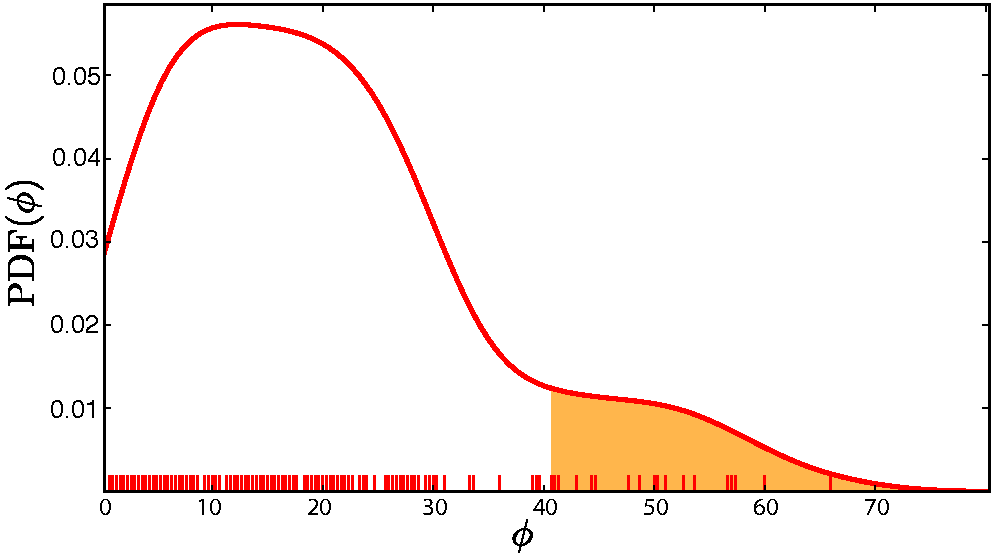
\includegraphics[width=\figSizeLarge]{ch03_general/pics/02_kernel_percentage_example.pdf}}
  \caption[Example of the Kernel Percentage Strategy for selecting which tags to recommend]{Example of the Kernel Percentage Strategy for selecting which tags to recommend (using $\percentageOfKernelPercentageStrategy = 0.05$). The curve represents the estimated $\probabilityDensityFunction$ of the scores of $\aggregatedCandidateTags$. Vertical markers on the horizontal axis show the actual positions of candidate tag scores. The shaded zone in the right of the figure corresponds to the 5\% of the total area of $\probabilityDensityFunction$. 
  Recommended tags are those under that zone.}
  \label{general:fig:kde_percentage_example}
\end{figure}

\begin{figure}
  \centerline{
  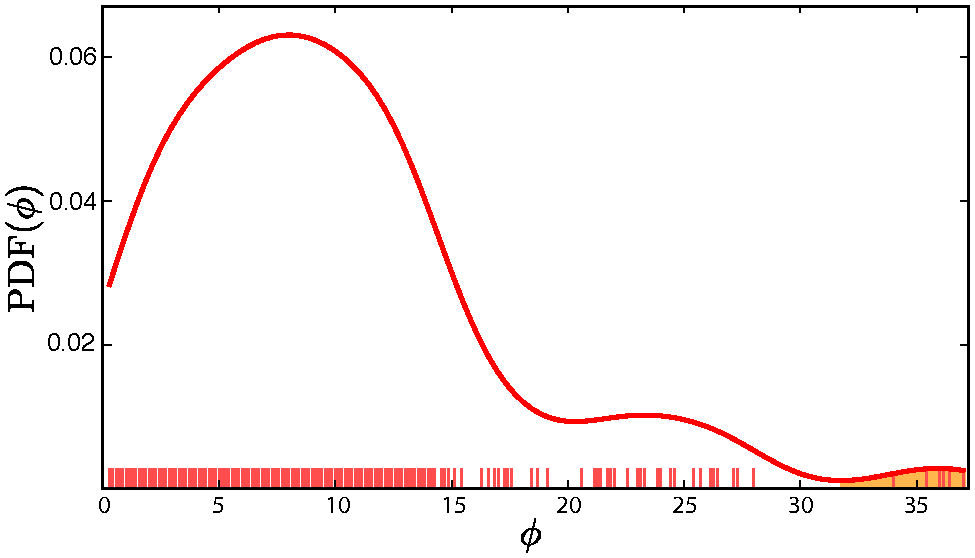
\includegraphics[width=\figSizeLarge]{ch03_general/pics/03_statistical_test_example.pdf}}
  \caption[Example of the Statistical Test Strategy for selecting which tags to recommend]{Example of the Statistical Test Strategy for selecting which tags to recommend. The curve represents the estimated $\probabilityDensityFunction$ of the scores of $\aggregatedCandidateTags$. Vertical markers on the horizontal axis show the actual positions of candidate tag scores. 
  Recommended tags are those under the shaded zone in the right. 
  In this example, the obtained threshold is $\scoreThreshold \approx 32$. Looking at the figure, it can be easily intuited that lower values of $\scoreThreshold$ would cause the statistical test of Eq.~\ref{general:eq:ad} to fail.}
  \label{general:fig:kde_example}
\end{figure}

\begin{figure}
  \centerline{
  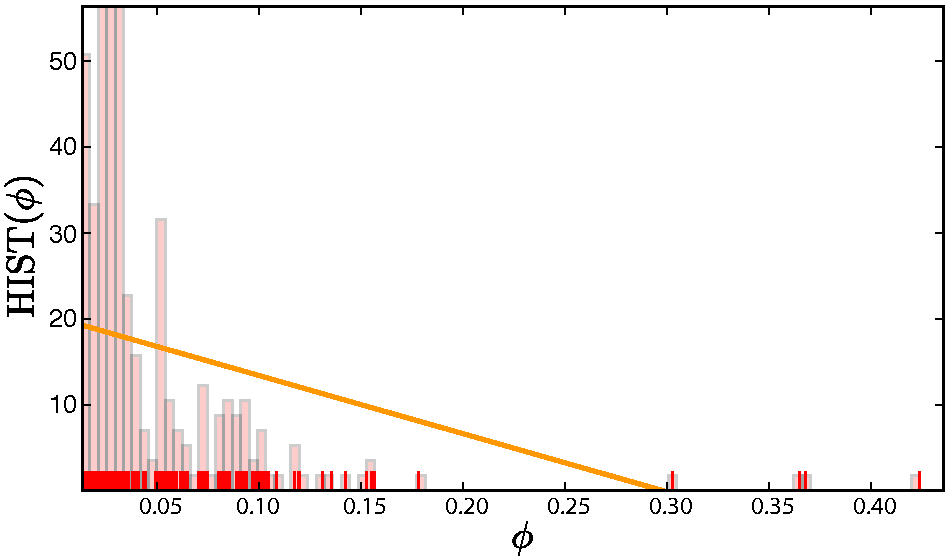
\includegraphics[width=\figSizeLarge]{ch03_general/pics/04_linear_regression_example.pdf}}
  \caption[Example of the Linear Regression Strategy for selecting which tags to recommend]{Example of the Linear Regression Strategy for selecting which tags to recommend. The straight line shows the linear regression of the histogram $\histogram$ of the scores of $\aggregatedCandidateTags$. Vertical markers on the horizontal axis show the actual positions of candidate tag scores. In this example, the obtained threshold is $\scoreThreshold \approx 0.29$, which is the point where the linear regression crosses the vertical axis. Recommended tags are those placed above 0.29.}
  \label{general:fig:polyfit_example}
\end{figure}


\subsubsection{Linear Regression Strategy}

The last strategy we propose consists in calculating the least-squares linear regression of the histogram $\histogram$ of $\scoreCandidateTag$. The threshold is set at the point where the linear regression crosses the vertical axis. 
The idea behind the Linear Regression Strategy is that, for a given $\histogram(\scoreCandidateTag)$, there will be a big concentration of candidate tags with low scores, and some outliers with bigger scores that will be separated from the rest (the most suitable tags for the recommendation). Thus, the linear regression will result in a straight line with a negative slope which will be useful to distinguish between both groups at the point where it crosses the vertical axis (Fig.~\ref{general:fig:polyfit_example}). The higher the concentration of low-scored candidates with respect to the outliers, the more pronounced the straight line will be, and the clearer the separation between both groups. 
Notice this strategy is also parameter-free.


\section{Evaluation}
\label{sec:general:evaluation_methodology}

From the combination of the different strategies above, we can define several tag recommendation methods which we evaluate through a tag prediction task (Sec.~\ref{sec:soa:evluation_of_tag_recommendation}). Essentially, what we do is to remove some tags from the resources of our datasets and then try to automatically predict them. In this section we describe the datasets and the methodology that we use for that evaluation.

\subsection{Datasets}
\label{sec:general:datasets}
We use two real-world datasets %(Table~\ref{tab:datasets}) 
collected from the tagging systems of Freesound and Flickr. In the case of Freesound, we consider all user annotations between April 2005 and September 2011, directly extracted from the Freesound database. From now on, we will refer to this dataset as \textsc{Freesound}. The Flickr data we use is a subset of photos taken in Barcelona, with user annotations performed approximately between January 2004 and December 2009. Flickr data was collected by~\cite{papadopoulos2010} and provided to us by the authors. To avoid confusion with the totality of the Flickr content, we will refer to the analysed Flickr subset as \textsc{Flickr1M}. Table~\ref{tab:datasets} shows some basic statistics about the folksonomies of both datasets.

\begin{table}
\begin{threeparttable}
\ra{1.2}
\footnotesize
  \begin{center}
    \makebox[0pt]{
    \begin{tabular}{@{}l@{\hskip 0.80cm}cc@{\hskip 0.5cm}cc@{}} %
      \toprule
      \multicolumn{1}{c}{} & \multicolumn{2}{c}{\textbf{Before filtering}} & \multicolumn{2}{c}{\textbf{After filtering}} \\ 
      \multicolumn{1}{c}{} & \textsc{Freesound} & \textsc{Flickr1M} & \textsc{Freesound} & \textsc{Flickr1M} \\ 
      \midrule
      Number of resources 		& 118,629 	& 107,617 	& 118,629 	& 107,617 \\ 
      Number of unique tags\tnote{a} 	& 33,790 	& 27,969 	& 6,232 	& 5,760 \\ 
      Number of contributor users\tnote{b} & 5,523 	& 5,463 	& 5,523 	& 5,463 \\ 
      Number of tag applications 	& 782,526	& 927,473 	& 730,417 	& 882,616 \\ 
      \bottomrule
    \end{tabular}
  }
    \begin{tablenotes}
    \item[a] Not necessarily semantically unique.
    \item[b] Users that have contributed by uploading, at least, one resource.
    \end{tablenotes}
  \caption[Basic statistics of the folksonomies of \textsc{Freesound} and \textsc{Flickr1M}]{Basic statistics of the folksonomies of \textsc{Freesound} and \textsc{Flickr1M} datasets. We see that the datasets feature comparable numbers. 
  The numbers under the ``After filtering'' column are computed by only considering tags that appear in at least 10 different resources (see below).}
  \label{tab:datasets}
  \end{center}
\end{threeparttable}
\end{table}

Freesound and Flickr have similar uploading processes in which users first provide the content (sounds and images, respectively) and then add as many tags as they feel appropriate to each resource\footnote{Since a software upgrade in 2011, Freesound requires a minimum of three tags to annotate a sound. However, the data we analyse is prior to the introduction of this requirement. In the case of Flickr, a single image can not be labeled with more than 75 tags, a large enough number not to be considered as a restriction for normal tagging behaviour.}. As opposed to other well-studied tagging systems such as Delicious or CiteULike, Freesound and Flickr feature a narrow folksonomy, meaning that resource annotations are shared among all users and, therefore, one single tag can only be assigned once to a particular resource (Sec.~\ref{sec:intro_tagging_systems_and_folksonomies}). Hence, we can not weigh the association between a particular tag and a resource by the number of times the same association has been performed by different users. 

\begin{figure}[t]
  \centerline{
  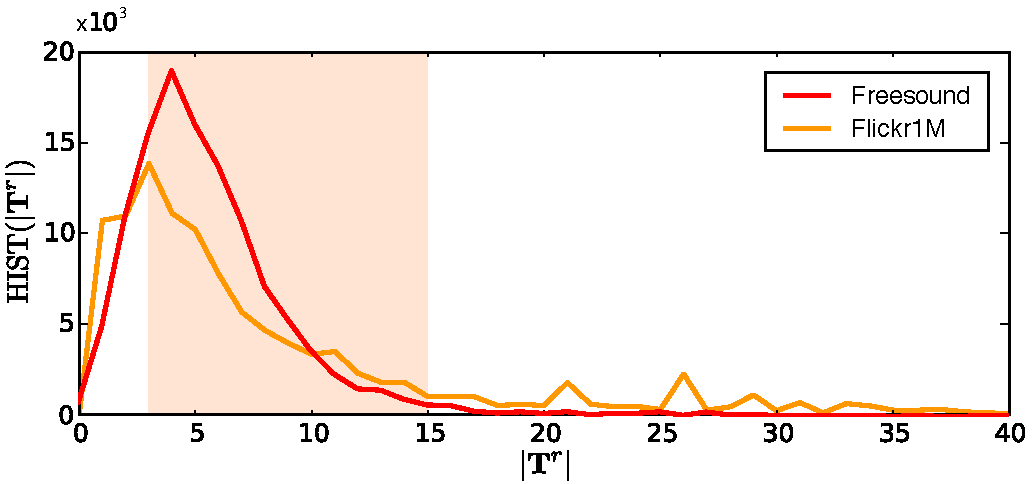
\includegraphics[width=\figSizeLarge]{ch03_general/pics/05_tag_distributions_B.pdf}}
  \caption[Histogram of the number of tags per resource in \textsc{Freesound} and \textsc{Flickr1M}]{Histogram of the number of tags per resource $|\tagsOfSoundR|$ in \textsc{Freesound} and \textsc{Flickr1M}. The average number of tags (standard deviation in parenthesis) per resource is 6.53 (6.47) and 7.50 (8.61) for \textsc{Freesound} and \textsc{Flickr1M}, respectively.}
  \label{general:fig:tag_distributions}
\end{figure}

The histogram of the number of tags per resource is qualitatively similar for the two datasets (Fig.~\ref{general:fig:tag_distributions}). We are particularly interested in recommending tags for resources that fall in the range of $|\tagsOfSoundR|=[3,15]$ tags, which are more than 80\% and 65\% of the total resources in \textsc{Freesound} and \textsc{Flickr1M}, respectively (Fig.~\ref{general:fig:tag_distributions}; shadowed zone). The reason for focusing on this range is that the tag recommendation scheme we propose takes as input the tags that have already been assigned to a resource. Thus, given the predictive nature of our evaluation (see below), we consider three tags as enough input information for our method to provide good recommendations. For resources with less than three tags, content-based strategies such as the ones outlined in Sec.~\ref{sec:soa:tag_recommendation_content_analysis} are probably more suited. On the other hand, we intuitively consider that resources with more than 15 tags are, in general, well enough described.

Among the set of all unique tags present in \textsc{Freesound} and \textsc{Flickr1M} folksonomies, we apply a threshold $\tagFrequencyThreshold=10$ to consider only the tags that have been used at least 10 times (i.e.,~tags that appear on at least 10 different resources). By this we assume that tags that have been used less than 10 times are irrelevant for our purposes. In addition, by discarding less frequent tags, we reduce the computational complexity of the calculation of $\similarityMatrix$ described in Step 1 (Sec.~\ref{sec:general:step1}). 
After applying this threshold, we are left with 6,232 unique tags in the \textsc{Freesound} folksonomy (representing approximately 20\% of the total) and with 5,760 unique tags in \textsc{Flickr1M} (also representing approximately 20\% of the total). This also means that we filter out all tag applications that do not associate any of these selected tags. Importantly, approximately 90\% of tag applications in both \textsc{Freesound} and \textsc{Flickr1M} involve one of these tags, thus we still take into account the vast majority of the original information (Table~\ref{tab:datasets}).


\subsection{Methodology}
\label{sec:general:evaluation_methodology_a}
Our evaluation methodology follows a standard information retrieval prediction task based on removing a number of tags from the resources of \textsc{Freesound} and \textsc{Flickr1M} and then trying to automatically predict them. The advantage of this approach is that it allows us to quickly evaluate the different recommendation algorithms without the need of human input. The main drawback is that tags that could be subjectively considered as good recommendations for a particular resource but are not present in the set of deleted tags, do not count as positive results. We mentioned this fact in Sec.~\ref{sec:soa:evluation_of_tag_recommendation} and further discuss it in Sec.~\ref{general:sec:discussion}.

For \textsc{Freesound} and \textsc{Flickr1M} datasets separately, we perform a 10-fold cross validation following the methodology described in~\cite{sal1997}. For each fold, we build $\similarityMatrix$ as described in Step 1, but only using the subset of the folksonomy corresponding to the training set of resources (i.e.,~only considering tag applications involving resources from the training set). For each resource in the evaluation set, we randomly delete a set of tags $\deletedTags$ from its originally assigned tags, yielding $\inputTags$, the input to our system. 
The number of tags we delete is chosen uniformly at random, with the only constraint that the length of $\inputTags$ must be maintained in the range of $|\inputTags|=[3,15]$ (see previous section). 
This constraint also implies that, in order to be able to remove at least one tag for each resource ($|\deletedTags| \geq 1$), we can only consider for evaluation resources with at least four tags. Furthermore, we add an upper limit to the number of tags and also filter out resources with more than 16 tags. We do that to avoid outliers with many tags which would result in very low recall values. 
Then, we run our tag recommendation methods using the tag similarity matrix $\similarityMatrix$ derived from the training set. 

Regarding evaluation measures, we compute $\precision$, $\recall$ and $\fmeasure$ as defined in Eq.~\ref{eq:prf_ch2} (Sec.~\ref{sec:soa:evluation_of_tag_recommendation}).
%for each individual resource according to
%\begin{equation}
%  \precision = \frac{|\recommendedTags \cap \deletedTags|}{|\recommendedTags|} \text{ }, \text{ }
%  \recall = \frac{|\recommendedTags \cap \deletedTags|}{|\deletedTags|} \text{ }, \text{ and }
%  \fmeasure = \frac{2\precision\recall}{\precision + \recall} \text{ ,}
%  \label{eq:prf_ch3}
%\end{equation}
%where $\recommendedTags$ is the set of recommended tags and $\deletedTags$ is the set of deleted tags. 
Then, global $\precision$, $\recall$ and $\fmeasure$ measures for each tag recommendation method are calculated by averaging $\precision$, $\recall$ and $\fmeasure$ across all resources evaluated with the particular recommendation method.
In addition to $\precision$, $\recall$ and $\fmeasure$, for each individual resource we also measure the number of recommended tags $|\recommendedTags|$. 
Evaluating $|\recommendedTags|$ is important because the longer the recommendation, the more comprehensive it potentially is, and the more difficult it is to maintain high precision values. We further discuss this aspect in Sec.~\ref{general:sec:discussion}. A general characterisation of the number of recommended tags per method is also obtained by averaging $|\recommendedTags|$ across all resources evaluated with a particular recommendation method.

\begin{table}
\begin{threeparttable}
  \ra{1.2}
  \begin{center}
  \footnotesize
  \makebox[0pt]{
    \begin{tabular}{@{}l@{\hskip 0.80cm}l@{\hskip 0.80cm}l@{}}
      \toprule
      \textbf{Name} & \textbf{Aggregation step} & \textbf{Selection step} \\
      \midrule
      \multicolumn{3}{c}{\emph{\rule{0pt}{4ex} Tag recommendation methods}}\\ 
      SimP@$\percentageOfPercentageStrategy$ & Similarity-based & Percentage ($\percentageOfPercentageStrategy=0.30$\tnote{a} , $\percentageOfPercentageStrategy=0.20$\tnote{b} )\\
      SimST & Similarity-based & Statistical Test \\ 
      SimKP@$\percentageOfKernelPercentageStrategy$ & Similarity-based & Kernel Percentage ($\percentageOfKernelPercentageStrategy=0.005$) \\ 
      SimLR & Similarity-based & Linear Regression\\ 
      RankP@$\percentageOfPercentageStrategy$ & Rank-based & Percentage ($\percentageOfPercentageStrategy=0.15$\tnote{a} , $\percentageOfPercentageStrategy=0.10$\tnote{b} )\\ 
      RankST & Rank-based & Statistical Test \\ 
      RankKP@$\percentageOfKernelPercentageStrategy$ & Rank-based & Kernel Percentage ($\percentageOfKernelPercentageStrategy=0.01$)\\ 
      RankLR & Rank-based & Linear Regression\\ 

      \multicolumn{3}{c}{\emph{\rule{0pt}{5ex} Baseline methods}}\\    
      BRankFIX@$\nRecommendedTagsInEvaluation$ & Rank-based & Fixed number ($\nRecommendedTagsInEvaluation \in [1,10]$) \\ 
      BSimFIX@$\nRecommendedTagsInEvaluation$ & Similarity-based & Fixed number ($\nRecommendedTagsInEvaluation \in [1,10]$) \\ %\cline{2-3}
      BRepeated@$\nRepeatedCandidateTags$ & \multicolumn{2}{c}{Repeated tags in all sets ${\candidateTagsPerInputTag}$($\nRepeatedCandidateTags \in [2,10]$)} \\ 
      BRandom & \multicolumn{2}{c}{Random replacement of $\recommendedTags$.} \\ 
      
      \multicolumn{3}{c}{\emph{\rule{0pt}{5ex} State of the art baseline methods}}\\ 
      GW@$\nRecommendedTagsInEvaluation$ & \cite{Garg2008} & Fixed number ($\nRecommendedTagsInEvaluation \in [1,10]$) \\ 
      SZ@$\nRecommendedTagsInEvaluation$ & \cite{Sigurbjornsson2008} & Fixed number ($\nRecommendedTagsInEvaluation \in [1,10]$) \\
      \bottomrule
    \end{tabular}
  }
  \begin{tablenotes}
    \item[a] Parameter settings for \textsc{Freesound} estimated in preliminary experiments. \item[b] Parameter settings for \textsc{Flickr1M} estimated in preliminary experiments.
  \end{tablenotes}
  \caption[List of evaluated tag recommendation methods]{Evaluated tag recommendation methods. All methods are evaluated using cosine similarity and $\nCandidateTagsPerInputTag=100$.}
  \label{tab:algorithms}
  \end{center}
\end{threeparttable}
\end{table}

Table~\ref{tab:algorithms} summarises all tag recommendation methods we evaluate. The first group of methods (Tag recommendation methods) are the eight possible combinations of aggregation and selection strategies that we propose. To avoid an intractable number of possible combinations, all methods are evaluated using only cosine similarity for Step 1, and setting $\nCandidateTagsPerInputTag=100$ (getting a maximum of 100 candidates for each input tag). 
We choose cosine similarity as default because of its widespread usage in the literature, and $\nCandidateTagsPerInputTag=100$ as an intuitively big enough number of candidates per input tag. 
We later study the influence of the chosen similarity measure and $\nCandidateTagsPerInputTag$, using only the highest performing methods of the main evaluation. For the methods that require the configuration of a percentage parameter (SimP@$\percentageOfPercentageStrategy$, SimKP@$\percentageOfKernelPercentageStrategy$, RankP@$\percentageOfPercentageStrategy$ and RankKP@$\percentageOfKernelPercentageStrategy$), we performed preliminary experiments with a subset of 10,000 resources from the main evaluation to determine the values of $\percentageOfPercentageStrategy$ and $\percentageOfKernelPercentageStrategy$ that reported higher average $\fmeasure$, and only consider these values in the main evaluation. 

Methods under the second group (Baseline methods, Table~\ref{tab:algorithms}) are simpler versions of the proposed methods that we use for comparative purposes. 
On the one hand, we compare with two methods that implement a very simple strategy for selecting which tags to recommend (Step 3) and always recommend the first $\nRecommendedTagsInEvaluation$ tags from $\aggregatedCandidateTags$, sorted by their scores (BRankFIX@$\nRecommendedTagsInEvaluation$ and BSimFIX@$\nRecommendedTagsInEvaluation$). We run these algorithms for values of $\nRecommendedTagsInEvaluation$ ranging from 1 to 10 and report only the best accuracy. 
Hence, the results reported for these methods constitute an upper bound of the accuracies that can be achieved when fixing the number of tags to recommend.
In preliminary experiments, we qualitatively observed a clear decrease of performance for values of $\nRecommendedTagsInEvaluation$ close to 10, therefore values $\nRecommendedTagsInEvaluation > 10$ are not considered (this also applies to other methods that have $\nRecommendedTagsInEvaluation$ as a parameter, see below).
On the other hand, we compare with an even simpler method (BRepeated@$\nRepeatedCandidateTags$) which, considering the union of all sets of candidates ${\candidateTagsPerInputTagOne}, {\candidateTagsPerInputTagTwo}, \text{... } \candidateTagsPerInputTag$ for a given resource, only recommends tags that are repeated more than $\nRepeatedCandidateTags$ times (independently of their scores). We run this algorithm for values of $\nRepeatedCandidateTags$ ranging from 2 to 10 and, as above, report only the best result found. 

We also compute a random baseline (BRandom) by replacing the set of $\recommendedTags$ with a random selection (of the same length) taken from $\aggregatedCandidateTags$. For each resource for which we recommend tags using any of the proposed methods above, we generate a random recommendation of the same length of $\recommendedTags$. Hence, for each proposed method, we also generate a randomised version of it. We take as the general random baseline the randomised version of all the proposed methods that reports higher $\fmeasure$.
Notice however, that these recommendations are not totally random: recommended tags are chosen from $\aggregatedCandidateTags$, not from the set of all possible tags in \textsc{Freesound} or \textsc{Flickr1M}. Moreover, by making a recommendation of the same length as the recommendation of the non-randomised version of the method, we preserve the distribution of the number of recommended tags for each method.

Finally, methods under the third group (State of the art methods, Table~\ref{tab:algorithms}) correspond to our implementations of the tag recommendation methods described by~\cite{Garg2008} and~\cite{Sigurbjornsson2008}, which we denote as GW and SZ, respectively. As these methods do not implement any selection step, we evaluate them for fixed values of $\nRecommendedTagsInEvaluation$ recommended tags ranging from 1 to 10 (and only report the best result found). \cite{Garg2008} describe several methods which contain different degrees of user personalisation. We implemented the ``global'' method which is not personalised and thus can be meaningfully compared to our methods. We implemented GW and SZ following the original references and set their parameters accordingly. 

\section{Results}
\label{sec:general:results}

\subsection{Recommendation accuracy}

From the average $\precision$, $\recall$ and $\fmeasure$ values for each one of the evaluated methods using the \textsc{Freesound} and \textsc{Flickr1M} datasets, we observe that Rank-based methods generally report higher $\fmeasure$ than Similarity-based methods (Tables~\ref{tab:results_freesound} and~\ref{tab:results_flickr}). Comparing the $\fmeasure$ values of each Rank-based method with its Similarity-based counterpart, we observe an average increase of 0.102 and 0.049 for \textsc{Freesound} and \textsc{Flickr1M}, respectively. We have assessed the statistical significance of this increase by performing pairwise Kruskal-Wallis tests~\citep{Corder2009} between the results of each Rank-based method and its Similarity-based counterpart, and all have shown to be statistically significant\footnote{In the rest of this chapter, in any comparison of $\fmeasure$ we indicate the results of the statistical significance tests as the maximum of the $\pvalue$-values of all pairwise comparisons.}, with a $\pvalue$-value several orders of magnitude below 0.01 (denoted as $\pvalue\ll0.01$). These results indicate that Step 2 (Aggregation of candidate tags) is better accomplished using the Rank-based Strategy.
% NOTE: statistical test was previously cited as wallis1952

Regarding the results of the different strategies for Step 3 (Selection of tags to recommend), we observe a very similar behaviour in \textsc{Freesound} and \textsc{Flickr\-1M} (Tables~\ref{tab:results_freesound} and~\ref{tab:results_flickr}, respectively). %That partially supports the generalisation of the proposed strategies to different kinds of data. 
In both datasets, methods using the Kernel Percentage Strategy (either with Rank-based or Similarity-based aggregation) perform significantly worse than the others, with an average $\fmeasure$ decrease of 0.036 for \textsc{Freesound} ($\pvalue\ll0.01$), and 0.048 for \textsc{Flickr1M} ($\pvalue\ll0.01$). Statistical Test, Linear Regression, and Percentage strategies report very similar $\fmeasure$, both in \textsc{Freesound} and \textsc{Flickr1M}, and specially in the case of Similarity-based aggregation. Nevertheless, the Percentage Strategy in combination with Rank-based aggregation provides the best obtained results in both datasets. When compared to the other selection strategies with Rank-based aggregation, it reports an average $\fmeasure$ increase of 0.025 for \textsc{Freesound} ($\pvalue\ll0.01$), and 0.039 for \textsc{Flickr1M} ($\pvalue\ll0.01$).
The similar results observed with \textsc{Freesound} and \textsc{Flickr1M} partially support the idea that the proposed methods are generalisable to different kinds of data.

\begin{table}[p] 
\ra{1.2}
\footnotesize
  \begin{center}
    \makebox[0pt]{
      \begin{tabular}{@{}lccc@{}}
      \toprule
  \multicolumn{4}{c}{\textsc{Freesound}} \\ 
  \textbf{Method} & \textbf{Precision} & \textbf{Recall} & \textbf{F-measure} \\ 
  \midrule
  RankP@0.15 & 0.444 & 0.532 & 0.437 \\ 
  RankST & 0.443 & 0.537 & 0.433 \\ 
  RankLR & 0.393 & 0.563 & 0.418 \\ 
  \textit{BRankFIX@2} & \textit{0.397} & \textit{0.468} & \textit{0.393} \\ 
  RankKP@0.01 & 0.352 & 0.524 & 0.383 \\ 
  \textit{GW@2} & \textit{0.375} & \textit{0.443} & \textit{0.371} \\ 
  SimLR & 0.347 & 0.397 & 0.324 \\
  SimP@0.30 & 0.344 & 0.414 & 0.323 \\ 
  SimST & 0.382 & 0.333 & 0.318 \\ 
  SimKP@0.005 & 0.356 & 0.294 & 0.294 \\ 
  \textit{BSimFIX@2} & \textit{0.303} & \textit{0.344} & \textit{0.293} \\ 
  \textit{SZ@2} & \textit{0.286} & \textit{0.334} & \textit{0.281} \\ 
  \textit{BRepeated@3} & \textit{0.176} & \textit{0.678} & \textit{0.235} \\ 
  \textit{BRandom (best)} & \textit{0.006} & \textit{0.033} & \textit{0.011} \\ 
  \bottomrule    
      \end{tabular}
    }  
    \caption[Average precision, recall and f-measure for tag recommendation methods using the \textsc{Freesound} dataset]{Average precision $\precision$, recall $\recall$ and f-measure $\fmeasure$ for tag recommendation methods using the \textsc{Freesound} dataset, sorted by f-measure. Baseline methods are marked in italics. For the sake of readability, we only show the results of baseline methods for the values of $\nRecommendedTagsInEvaluation$ and $\nRepeatedCandidateTags$ that reported higher f-measure.}
  \label{tab:results_freesound}
  \end{center}
\end{table}

\begin{table}[p] 
\ra{1.2}
\footnotesize
  \begin{center}
    \makebox[0pt]{
      \begin{tabular}{@{}lccc@{}}
      \toprule
  \multicolumn{4}{c}{\textsc{Flickr1M}} \\ 
  \textbf{Method} & \textbf{Precision} & \textbf{Recall} & \textbf{F-measure} \\ 
  \midrule
  RankP@0.10 & 0.503 & 0.513 & 0.452 \\ 
  \textit{GW@2} & \textit{0.480} & \textit{0.517} & \textit{0.442} \\ 
  \textit{BRankFIX@2} & \textit{0.475} & \textit{0.511} & \textit{0.441} \\ 
  RankST & 0.459 & 0.556 & 0.437 \\ 
  RankLR & 0.384 & 0.597 & 0.414 \\ 
  SimP@0.20 & 0.462 & 0.422 & 0.394 \\ 
  RankKP@0.01 & 0.389 & 0.483 & 0.388 \\ 
  SimST & 0.475 & 0.340 & 0.384 \\ 
  SimLR & 0.412 & 0.461 & 0.384 \\ 
  \textit{BSimFIX@2} & \textit{0.417} & \textit{0.440} & \textit{0.382} \\ 
  \textit{SZ@2} & \textit{0.384} & \textit{0.410} & \textit{0.353} \\ 
  SimKP@0.005 & 0.430 & 0.325 & 0.339 \\ 
  \textit{BRepeated@3} & \textit{0.163} & \textit{0.715} & \textit{0.219} \\ 
  \textit{BRandom  (best)} & \textit{0.007} & \textit{0.045} & \textit{0.020} \\    \bottomrule
      \end{tabular}
    }
    \caption[Average precision, recall and f-measure for tag recommendation methods using the \textsc{Flickr1M} dataset]{Average precision $\precision$, recall $\recall$ and f-measure $\fmeasure$ for tag recommendation methods using the \textsc{Flickr1M} dataset, sorted by f-measure. Baseline methods are marked in italics. For the sake of readability, we only show the results of baseline methods for the values of $\nRecommendedTagsInEvaluation$ and $\nRepeatedCandidateTags$ that reported higher f-measure.}
  \label{tab:results_flickr}
  \end{center} 
\end{table}

Having a look at the results of the baseline methods based on recommending a fixed number of tags (BRankFIX@$2$ and BSimFIX@$2$) we can see that, in terms of $\fmeasure$, they perform very similarly to the other proposed methods, and in some cases even outperform them (especially in the \textsc{Flickr1M} dataset). Importantly, we have to take into account that these baseline methods only vary from our proposed methods in the last step of the recommendation process, and that their reported results correspond to the upper bound of their performance (Sec.~\ref{sec:general:evaluation_methodology_a}). 
That good performance thus points out the effectiveness of the first two steps of the method in promoting the most relevant tags on the first positions of the list of candidates. If we compare these baseline methods with the state of the art implementations (GW@$2$ and SZ@$2$), we can see that our baselines get nearly equal or significantly higher $\fmeasure$ than those.
Regarding the other baselines, BRepeated@$\nRepeatedCandidateTags$ reports very low results both in \textsc{Freesound} and \textsc{Flickr1M} datasets, and BRandom baseline remains significantly below all the other methods.


\subsection{Number of recommended tags}

Another aspect to evaluate from the tag recommendation methods is the number of tags that they recommend $|\recommendedTags|$. 
Table~\ref{tab:number_of_recommended_tags} shows the average $|\recommendedTags|$ for the evaluated methods using the \textsc{Freesound} and \textsc{Flickr1M} datasets. We consider that methods which recommend higher number of tags and maintain overall high precision values are the most valuable for our purposes, as they provide both comprehensive and appropriate tag recommendations (i.e.,~relevant tags for the particular resource). 
In general we see that the best scoring methods, corresponding to the first positions of the table, recommend more tags than BRankFIX@2 and GW@2 (Table~\ref{tab:number_of_recommended_tags}), and at the same time report higher (or very similar) precision values and overall f-measure (see Tables~\ref{tab:results_freesound} and~\ref{tab:results_flickr}). If we look at the evaluation results obtained with BRankFIX@$\nRecommendedTagsInEvaluation$ methods when recommending more than two tags, we observe significant drops in precision ($\precision=0.323$ for $\nRecommendedTagsInEvaluation=3$ and $\precision=0.272$ for $\nRecommendedTagsInEvaluation=4$ in \textsc{Freesound}, and $\precision=0.391$ for $\nRecommendedTagsInEvaluation=3$ and $\precision=0.333$ for $\nRecommendedTagsInEvaluation=4$ in \textsc{Flickr1M}). Similar precision drops are observed in GW@$\nRecommendedTagsInEvaluation$ ($\precision=0.306$ for $\nRecommendedTagsInEvaluation=3$ and $\precision=0.257$ for $\nRecommendedTagsInEvaluation=4$ in \textsc{Freesound}, and $\precision=0.396$ for $\nRecommendedTagsInEvaluation=3$ and $\precision=0.340$ for $\nRecommendedTagsInEvaluation=4$ in \textsc{Flickr1M}).
This further highlights the superiority of our proposed methods over the baselines.

It is also interesting to see that the number of recommended tags is not only driven by the selection strategy of Step 3, but also depends on the type of aggregation used in Step 2. Both in \textsc{Freesound} and \textsc{Flickr1M}, we observe that when using Rank-based aggregation, highest $|\recommendedTags|$ is obtained using the strategy of Linear Regression for selecting which tags to recommend (followed by Statistical Test, Percentage and Kernel Percentage strategies). 
However, when using Similarity-based aggregation, the highest $|\recommendedTags|$ is obtained with the Percentage Strategy, followed by Linear Regression, Statistical Test and Kernel Percentage strategies  (Table~\ref{tab:number_of_recommended_tags}). This shows that the selection strategies behave differently if the scores of $\aggregatedCandidateTags$ are ranks or similarity values. In general, Rank-based methods recommend more tags than their Similarity-based counterparts, with an average $|\recommendedTags|$ increase of 0.38 for \textsc{Freesound} ($\pvalue\ll0.01$), and 0.86 for \textsc{Flickr1M} ($\pvalue\ll0.01$).
Given that Rank-based aggregation methods also report higher $\fmeasure$, this reinforces the aforementioned observation that Step 2 is better accomplished using the Rank-based Strategy.

\begin{table} \footnotesize
  \begin{center}
  \ra{1.2}
    \makebox[0pt]{
      \begin{tabular}{@{}lc@{\hskip 1cm}lc@{}}
      \toprule
  \multicolumn{2}{c}{\textsc{Freesound}} & \multicolumn{2}{c}{\textsc{Flickr1M}} \\ 
  \textbf{Method} & \textbf{$|\recommendedTags|$} & \textbf{Method} & \textbf{$|\recommendedTags|$} \\ 
  \midrule
  RankP@0.15 & 3.03 (2.60) & RankP@0.10 & 2.68 (1.96) \\ 
  RankST &  3.36 (3.30) & \emph{GW@2} &  \emph{2.00 (0.00)} \\ 
  RankLR &  3.55 (7.14) & \emph{BRankFIX@2} & \emph{2.00 (0.00)} \\ 
  \emph{BRankFIX@2} & \emph{2.00 (0.00)} & RankST & 3.96 (3.64) \\ 
  RankKP@0.01 & 2.89 (1.29) & RankLR & 4.64 (4.25) \\ 
  \emph{GW@2} &  \emph{2.00 (0.00)} & SimP@0.20 & 3.97 (1.64) \\    
  SimLR & 3.42 (2.36) & RankKP@0.01 & 2.60 (1.47) \\ 
  SimP@0.30 & 4.06 (3.10) & SimST & 1.98 (1.70) \\ 
  SimST & 2.35 (2.17) & SimLR & 3.15 (2.16) \\  
  SimKP@0.05 & 1.47 (0.70) & \emph{BSimFIX@2} & \emph{2.00 (0.00)} \\   
  \emph{BSimFIX@2} & \emph{2.00 (0.00)} & \emph{SZ@2} &  \emph{2.00 (0.00)} \\ 
  \emph{SZ@2} &  \emph{2.00 (0.00)} & SimKP@0.05 & 1.35 (0.73) \\ 
  \emph{BRepeated@3} & \emph{5.17 (8.17)} & \emph{BRepeated@3} & \emph{4.27 (3.11)} \\ 
  \emph{BRandom (best)} & \emph{5.17 (8.17)} & \emph{BRandom (best)} & \emph{4.27 (3.11)} \\ 
  \bottomrule
      \end{tabular}
    } 

    \caption[Average number of recommended tags per tag recommendation method]{Average number of recommended tags $|\recommendedTags|$ for tag recommendation methods using the \textsc{Freesound} and \textsc{Flickr1M} datasets (standard deviation into parentheses). Methods are displayed and sorted according to the $\fmeasure$ values of Tables~\ref{tab:results_freesound} and ~\ref{tab:results_flickr}. Baseline methods are marked in italics. } 
    %\vspace{0.8cm}
  
  \label{tab:number_of_recommended_tags} 
  \end{center}
\end{table}


\begin{figure}[t]
  \centering
  \subbottom[]{
    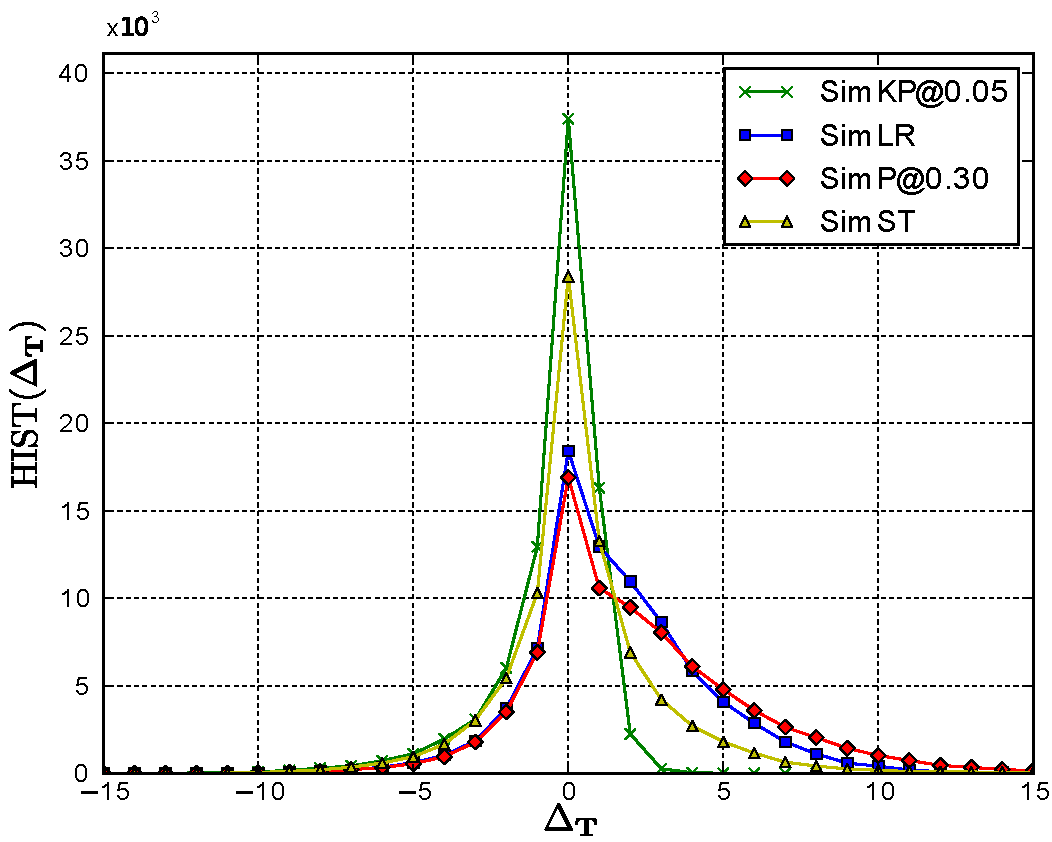
\includegraphics[width=\figSizeMid]{ch03_general/pics/06_similarity_based_hist2.pdf}}
  \subbottom[]{
    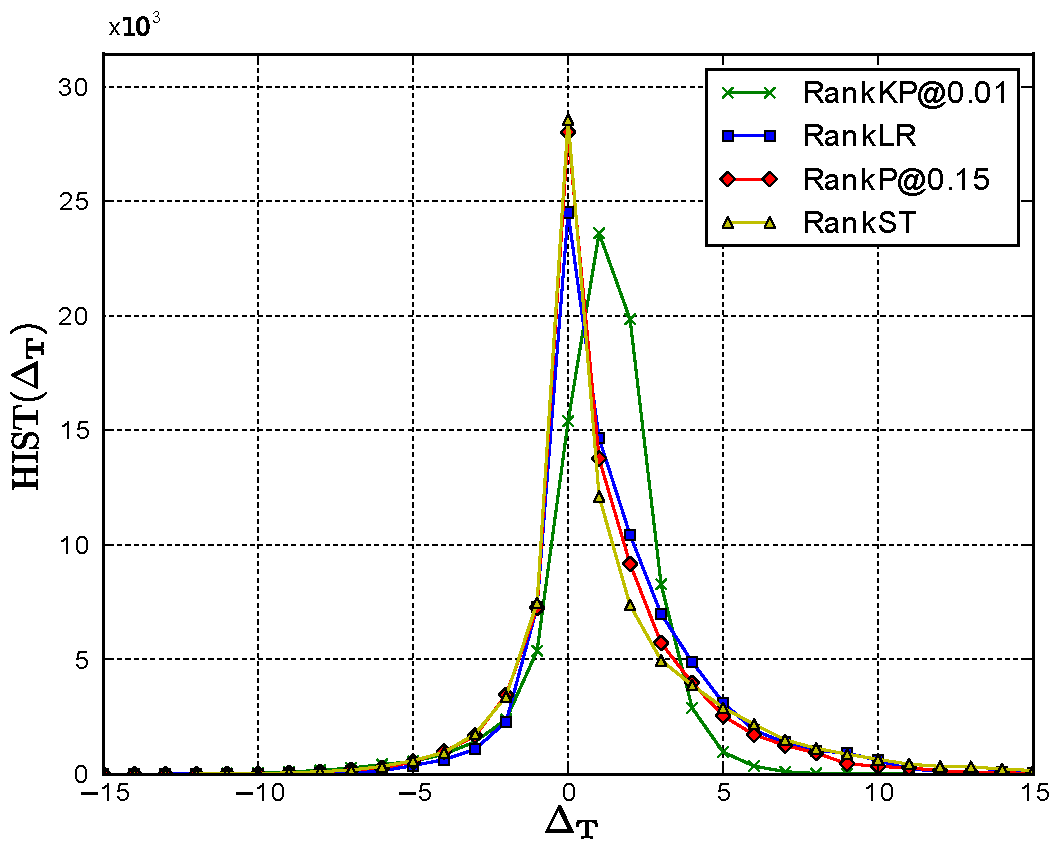
\includegraphics[width=\figSizeMid]{ch03_general/pics/07_rank_based_hist2.pdf}}
  \caption[Histogram of the difference between the number of recommended tags and the number of deleted tags]{Histogram of the difference between the number of recommended tags and the number of deleted tags $\differenceNRecTagsAndNDelTags$ for Similarity-based (a) and Rank-based (b) tag recommendation methods using \textsc{Freesound} dataset. Qualitatively similar results were obtained with \textsc{Flickr1M}.}
  \label{general:fig:hist}
\end{figure}

Furthermore, we also looked at the difference between the number of recommended tags and the number of tags that are deleted for each resource ($\differenceNRecTagsAndNDelTags = |\recommendedTags| - |\deletedTags|$). 
In Fig.~\ref{general:fig:hist} we show the histogram of $\differenceNRecTagsAndNDelTags$ for our proposed methods. We observe that most of our proposed methods report the maximum peak of the histogram at $\differenceNRecTagsAndNDelTags = 0$ (Fig.~\ref{general:fig:hist}). This suggests that these methods have a certain tendency to recommend as many tags as have been removed. 
Although it is not the goal of the tag recommendation methods to recommend the exact number of tags that have been removed (actually, this measure only makes sense under our tag prediction task-based evaluation), the results shown here are an interesting indicator that our proposed methods are able to indirectly estimate the number of deleted tags given only a set of input tags and the information embedded in the folksonomy. A plot of the average number of recommended tags as a function of the number of input tags and the number of deleted tags further supports this conclusion (Fig.~\ref{general:fig:added}). We can qualitatively observe how $|\recommendedTags|$ grows along with $|\deletedTags|$, specially for low $|\inputTags|$. 
It can also be observed that there is a tendency of $|\recommendedTags|$ increasing when $|\inputTags|$ decreases, meaning that the smaller the number of input tags, the more tags are recommended. 
Similar plots can be obtained with the other proposed recommendation methods, specially for RankLR and RankP (both in \textsc{Freesound} and \textsc{Flickr1M} datasets).


\subsection{Other relevant aspects}

In order to better understand the behaviour of the proposed tag recommendation methods, we have carried out further analyses on the influence of particular aspects of the methods. To avoid very intensive computation we have only focused on the three methods that report best average $\fmeasure$ both in \textsc{Freesound} and \textsc{Flickr1M}, that is to say, RankST, RankLR and RankP@$\percentageOfPercentageStrategy$ (with $\percentageOfPercentageStrategy$ being 0.15 for \textsc{Freesound} and 0.10 for \textsc{Flickr1M} as shown in Table \ref{tab:algorithms}). In the following sections we report experiments concerning these aspects.

\begin{figure}
  \centerline{
  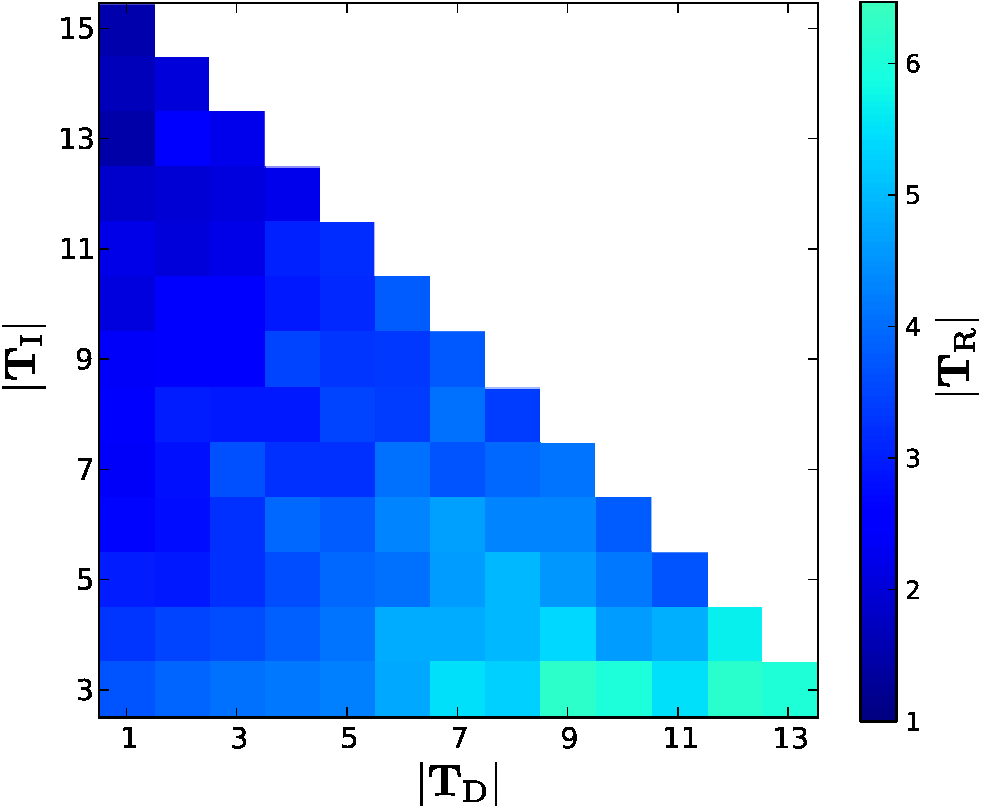
\includegraphics[width=\figSizeMid]{ch03_general/pics/08_recommended_tags_statistical_test.pdf}} 
  \caption[Average number of recommended tags as a function of the number of input tags and the number of deleted tags]{Average number of recommended tags $|\recommendedTags|$ as a function of  the number of input tags $|\inputTags|$ and the number of deleted tags $|\deletedTags|$, for method RankST and \textsc{Freesound} dataset.}
  \label{general:fig:added}
\end{figure}

\subsubsection{Limiting the minimum number of input tags}

To assess the influence of limiting the number of input tags, we now repeat the main experiments but include resources evaluated with less than three input tags. 
As it could be expected, we obtain lower $\fmeasure$ scores (Table \ref{tab:results_no_filt}).
On average, all methods have a decrease in $\fmeasure$  of 0.154 ($\pvalue\ll0.01$) and 0.141 ($\pvalue\ll0.01$) for \textsc{Freesound} and \textsc{Flickr1M} datasets, respectively. This confirms our initial observation that content-based methods might be more suited to recommend tags to scarcely labeled resources. In Fig.~\ref{general:fig:3d} we have plotted average $\fmeasure$ as a function of the number of input tags and the number of deleted tags for the RankP@0.15 method (using the \textsc{Freesound} dataset). This plot is useful to understand in which range of the number of input tags and number of deleted tags the recommendation performs better.  As it can be observed, the optimum conditions for high $\fmeasure$ are found with 5 or more input tags and 6 or less deleted tags, meaning that the recommendation needs a few input tags to effectively aggregate and select candidates and not many tags to predict.
Nevertheless, the fact that $\fmeasure$ is way above the random baseline of Tables~\ref{tab:results_freesound} and~\ref{tab:results_flickr} emphasizes that, even outside the optimum conditions, the proposed methods are still useful to some extent.


\begin{table} \footnotesize
\ra{1.2}
  \begin{center}
    \makebox[0pt]{
      \begin{tabular}{@{}lccc@{}}
      \toprule
	\textbf{Method} & \textbf{Precision} & \textbf{Recall} & \textbf{F-measure} \\  
	\midrule
  \multicolumn{4}{c}{\rule{0pt}{3ex}\textsc{Freesound}} \\ 
  
	RankP@0.15 & 0.323 & 0.375 & 0.297 \\  
	RankST & 0.337 & 0.326 & 0.285 \\  
	RankLR & 0.252 & 0.336 & 0.244 \\ 
	\multicolumn{4}{c}{\rule{0pt}{3ex}\textsc{Flickr1M}} \\ 
	RankST & 0.394 & 0.377 & 0.326 \\  
	RankP@0.10 & 0.329 & 0.434 & 0.309 \\  
	RankLR & 0.244 & 0.352 & 0.243 \\ 
  \bottomrule
      \end{tabular}
    }
    \caption[Average precision, recall and f-measure for the best scoring methods without filtering the number of input tags]{Average precision $\precision$, recall $\recall$ and f-measure $\fmeasure$ for the best scoring methods in \textsc{Freesound} and \textsc{Flickr1M} without filtering the number of input tags. Results are sorted in descending $\fmeasure$. }
    \label{tab:results_no_filt}
  \end{center}
\end{table}

\begin{figure}
  \centering
  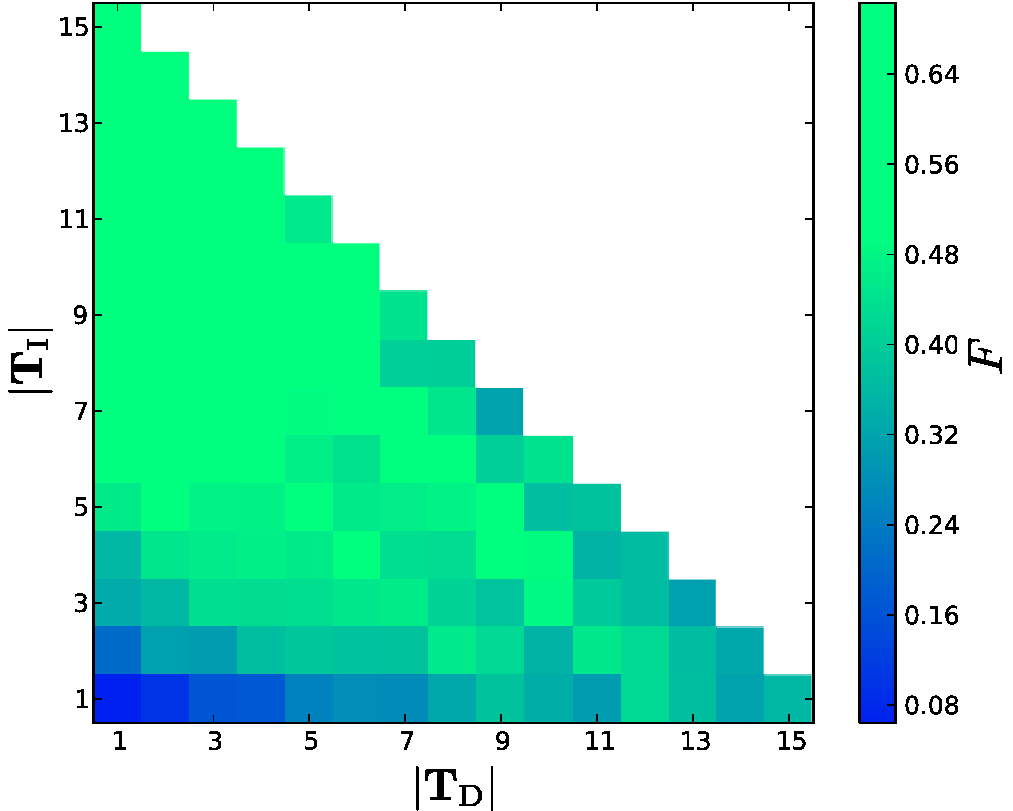
\includegraphics[width=\figSizeMid]{ch03_general/pics/09_fmeasure_percentage.pdf} 
  \caption[Average f-measure as a function of  the number of input tags and the number of deleted tags]{
  Average f-measure $\fmeasure$ as a function of  the number of input tags $|\inputTags|$ and the number of deleted tags $|\deletedTags|$ for method  RankP@0.15 and \textsc{Freesound} dataset. This plot includes the results of resources evaluated with fewer than three input tags.}
  \label{general:fig:3d}
\end{figure}


\subsubsection{Using alternative similarity measures}

As has been explained in the evaluation methodology, all previously reported experiments have been performed using cosine similarity as the similarity measure for Step 1. 
In this subsection we repeat the evaluation for the best scoring methods but now using Jaccard and tag co-occurrence as similarity measures (Table~\ref{tab:sims}). In both datasets and for all methods, cosine similarity is the metric that obtains higher $\fmeasure$, with an average increase of 0.009 ($\pvalue\ll0.01$, \textsc{Freesound}) and 0.053 ($\pvalue\ll0.01$, \textsc{Flickr1M}) respect to Jaccard, and 0.086 ($\pvalue\ll0.01$, \textsc{Freesound}) and 0.108 ($\pvalue\ll0.01$, \textsc{Flickr1M}) respect to tag co-occurrence. In the case of \textsc{Freesound}, we observe that the difference between cosine and Jaccard similarity is very small, and could be due to a marginal increase in the average number of recommended tags, thus lowering precision and getting a higher number of wrong recommendations. In \textsc{Flickr1M} the increase in the average number of recommended tags is more prominent, and so is the decrease in $\fmeasure$ for the methods using Jaccard distance.
We have observed that performing the same experiment with the Similarity-based counterparts of these methods (SimP@$\percentageOfPercentageStrategy$, SimST and SimLR) also leads to very similar results, with cosine similarity obtaining the highest $\fmeasure$ followed by Jaccard and tag co-occurrence. However, $\fmeasure$ differences among the different similarity measures tend to be slightly larger than these obtained with Rank-based methods.


\begin{table} \footnotesize
\ra{1.1}
  \begin{center}
  \makebox[0pt]{
    \begin{tabular}{@{}lcccc@{}}
    \toprule
      \textbf{Method} & \textbf{Precision} & \textbf{Recall} & \textbf{F-measure} & \textbf{$|\recommendedTags|$} \\ 
      \midrule
      \multicolumn{5}{c}{\rule{0pt}{4ex}\textsc{Freesound}} \\ 
      \multicolumn{5}{c}{\rule{0pt}{2ex} \emph{Cosine similarity}} \\ 
      RankP@0.15 & 0.444 & 0.532 & \textbf{0.437} & 3.03 \\ 
      RankST & 0.443 & 0.537 & 0.433 & 3.36 \\ 
      RankLR & 0.393 & 0.563 & 0.418 & \textbf{3.55} \\ 

      \multicolumn{5}{c}{\rule{0pt}{2ex} \emph{Jaccard similarity}} \\ 
      RankP@0.15 & 0.425 & 0.543 & \textbf{0.431} & 3.28 \\ 
      RankST & 0.421 & 0.552 & 0.423 & \textbf{3.91} \\ 
      RankLR & 0.370 & 0.570 & 0.405 & 3.84 \\ 

      \multicolumn{5}{c}{\rule{0pt}{2ex} \emph{Tag co-ocurrence}} \\ 
      RankP@0.15 & 0.339 & 0.483 & \textbf{0.352} & 3.37 \\ 
      RankST & 0.336 & 0.492 & 0.348 & 3.85 \\ 
      RankLR & 0.284 & 0.541 & 0.330 & \textbf{4.65} \\ 

      \multicolumn{5}{c}{\rule{0pt}{4ex}\textsc{Flickr1M}} \\ 
      \multicolumn{5}{c}{\rule{0pt}{2ex} \emph{Cosine similarity}} \\ 
      RankP@0.10 & 0.503 & 0.513 & \textbf{0.452} & 2.68 \\ 
      RankST & 0.459 & 0.556 & 0.437 & 3.96 \\ 
      RankLR & 0.384 & 0.597 & 0.414 & \textbf{4.64} \\ 

      \multicolumn{5}{c}{\rule{0pt}{2ex} \emph{Jaccard similarity}} \\ 
      RankP@0.10 & 0.417 & 0.491 & \textbf{0.397} & 3.46 \\ 
      RankST & 0.374 & 0.555 & 0.378 & \textbf{5.97} \\ 
      RankLR & 0.336 & 0.561 & 0.369 & 5.35 \\ 

      \multicolumn{5}{c}{\rule{0pt}{2ex} \emph{Tag co-ocurrence}} \\ 
      RankP@0.10 & 0.346 & 0.458 & \textbf{0.337} & 3.77 \\ 
      RankST & 0.320 & 0.505 & 0.329 & 5.43 \\ 
      RankLR & 0.269 & 0.542 & 0.311 & \textbf{6.12} \\ 
      \bottomrule
    \end{tabular}
  }
  \caption[Average precision, recall, f-measure and number of recommended tags using different similarity measures]{Average precision $\precision$, recall $\recall$, f-measure $\fmeasure$ and number of recommended tags $|\recommendedTags|$, using different similarity measures.}
  \label{tab:sims}
  \end{center}
\end{table}


\subsubsection{Number of candidate tags per input tag}

In order to understand the effect of the number of candidates per input tag $\nCandidateTagsPerInputTag$ (Step 1), we have performed a series of experiments with the best scoring methods. Similar to the main experiments described in Sec.~\ref{sec:general:evaluation_methodology_a}, we have performed 10-fold cross validations for each one of the best scoring methods, giving different values to $\nCandidateTagsPerInputTag$. To speed up computation time, we limited the number of resources of each experiment to 10,000. The rest of the parameters have remained constant (input tags in the range of $[3,15]$, using cosine similarity, and $\percentageOfPercentageStrategy=0.15$ or $0.10$ for \textsc{Freesound} and \textsc{Flickr1M}, respectively). The results show that most of the methods achieve a local maxima in the range of $\nCandidateTagsPerInputTag=[75,150]$, and then show a very slow decaying tendency (Fig.~\ref{general:fig:ns}). In \textsc{Freesound}, RankP@0.15 and RankST are shown to be more constant, without a 
noticeable decay (standard deviation of 0.005 for both RankST and RankP in the range of $\nCandidateTagsPerInputTag=[125,400]$). These results suggest that after selecting a sufficient amount of $\nCandidateTagsPerInputTag$ candidates for each input tag, the most relevant tags have already been selected, and increasing $\nCandidateTagsPerInputTag$ does not have a relevant impact on the output of the recommendation as score values for the ``extra'' candidates are generally low. 
According to Fig.~\ref{general:fig:ns}, for most of the methods, highest $\fmeasure$ is obtained with $\nCandidateTagsPerInputTag\approx 125$, which is slightly higher than the value we used for our main experiments ($\nCandidateTagsPerInputTag=100$). However, the average $\fmeasure$ increase is less than 1\%, and significance tests fail with $\pvalue \approx 0.10$ when comparing the methods configurations with $\nCandidateTagsPerInputTag=100$ and $\nCandidateTagsPerInputTag=125$.

\begin{figure}[t]
  \centerline{
  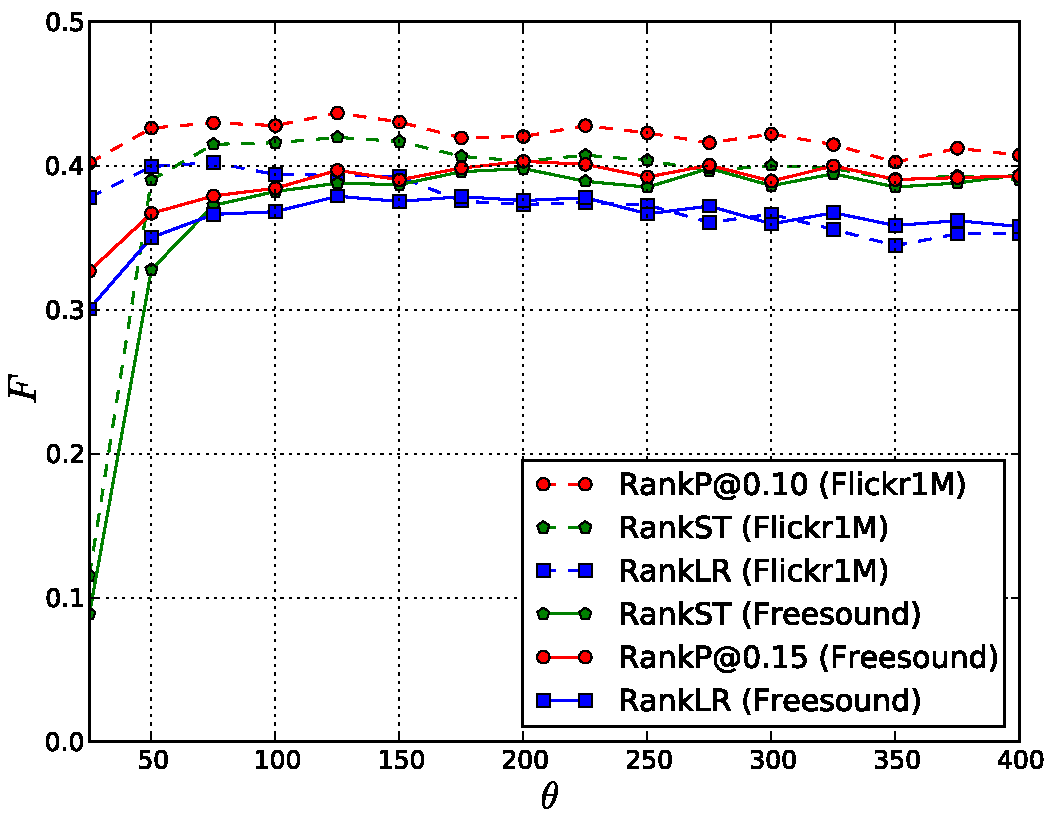
\includegraphics[width=\figSizeMid]{ch03_general/pics/10_fmeasure_per_N.pdf}}
  \caption[Average f-measure for different numbers of candidate tags per input tag]{Average f-measure $\fmeasure$ with different values of $\nCandidateTagsPerInputTag$ for the best scoring recommendation methods in \textsc{Freesound} and \textsc{Flickr1M} (each experiment performed with 10,000 resources).}
  \label{general:fig:ns}
\end{figure}

\subsubsection{Contribution of each step of the recommendation scheme}

To finish our analysis, we perform several experiments to evaluate the contribution of each step of the proposed tag recommendation scheme. For the best scoring methods, we have repeated the 10-fold cross validations of the main experiments three times, replacing in each run one step of the recommendation system by a randomised version of itself.
In the first run, we have replaced Step 1 by a random version that, for each input tag, selects $\nCandidateTagsPerInputTag$ random candidates from the whole vocabulary of the folksonomy (using $\nCandidateTagsPerInputTag=100$). 
In the second run we have maintained Step 1 as in the original setting, but have replaced Step 2 by an alternative version that, after performing a Rank-based aggregation, detaches the score values from each candidate in $\aggregatedCandidateTags$, and randomly re-assigns them among the candidates. 
Finally, in the third run of the experiments, we have maintained Steps 1 and 2 as in the original setting, but replaced the selection step by an alternative version that recommends the first $\nRecommendedTagsInEvaluation$ tags from $\aggregatedCandidateTags$ (sorted by the scores of candidates). In that case, $\nRecommendedTagsInEvaluation$ is determined by a random number generator with a normal distribution with the same mean ($\gaussianMean$) and standard deviation ($\gaussianStDev$) as that observed for the number of deleted tags in the main experiments ($\gaussianMean = 1.92$ and $\gaussianStDev = 1.58$ for \textsc{Freesound}, and $\gaussianMean = 2.32$ and $\gaussianStDev = 2.01$ for \textsc{Flickr1M}). By applying the distribution of the number of deleted tags to the number of recommended tags, we optimize $\fmeasure$ scores as precision and recall errors are minimised when $\differenceNRecTagsAndNDelTags \approx 0$.

Runs 1 and 2 report very low $\fmeasure$ in both datasets (Table~\ref{tab:random}). Run 3 obtains quite acceptable results, but with an average $\fmeasure$ decrease of 0.1270 ($\pvalue\ll0.01$, \textsc{Freesound}) and 0.1214 ($\pvalue\ll0.01$, \textsc{Flickr1M}) with respect to the normally working methods (without any randomisation). Hence, run 3 is still far from the optimum recommendation of normally working methods (Table~\ref{tab:random}). Given that Steps 1 and 2 are tightly coupled, failing in any of them has a very important impact on the final results. In the case of randomising Step 1, further steps can not effectively recommend tags as the original candidates are not relevant. When randomising Step 2, although candidate tags obtained in Step 1 are relevant, the aggregation can not assign meaningful scores to the candidates and thus the selection step fails in selecting which tags to recommend. Finally, when randomising Step 3, although a meaningful list of candidates can be sorted with meaningful score 
values, the number of tags that is recommended for each resource is selected in a completely unrelated way with respect to the score distribution of the candidates, thus not considering the possible relevance of each candidate given the other candidates. Overall, this demonstrates the usefulness of each of the three proposed steps in our tag recommendation scheme.

\begin{table} \footnotesize
\ra{1.2}
  \begin{center}
  \makebox[0pt]{
    \begin{tabular}{@{}l@{\hskip 1.0cm}cccc@{}}
    \toprule
      \multicolumn{1}{l}{\textbf{Method}} & \textbf{Run 1} & \textbf{Run 2} & \textbf{Run 3} & \textbf{No rand.} \\  %\textbf{No randomisation} \\ 
      \midrule
      \multicolumn{5}{c}{\rule{0pt}{3ex} \textsc{Freesound}} \\ 
      RankP@0.15 & $<$ 0.001 & 0.012 & 0.303 & 0.437 \\ 
      RankST & $<$ 0.001 & 0.006 & 0.302 & 0.433 \\ 
      RankLR & $<$ 0.001 & 0.007 & 0.302 & 0.418 \\ 
      \multicolumn{5}{c}{\rule{0pt}{3ex} \textsc{Flickr1M}} \\ 
      RankP@0.10 & $<$ 0.001 & 0.018 & 0.313 & 0.452 \\ 
      RankST & $<$ 0.001 & 0.010 & 0.313 & 0.437 \\ 
      RankLR & $<$ 0.001 & 0.011 & 0.312 & 0.414 \\ 
      \bottomrule
    \end{tabular}
  }
  \caption[Average f-measures after randomising steps of the best scoring tag recommendation methods]{Average f-measures $\fmeasure$ after randomising steps 1, 2 and 3 of the best scoring tag recommendation methods in \textsc{Freesound} and \textsc{Flickr1M}. The ``No rand.'' column shows the performance of the recommendation methods when no steps are randomised.}
  \label{tab:random}
  \end{center}
\end{table}

\section{Conclusion and discussion}
\label{general:sec:discussion}

In this chapter we have presented a general scheme for tag recommendation systems based on tag co-occurrence in folksonomies. This scheme is composed of three steps for which we have proposed different strategies. Step 1, Candidate tag selection, selects a number of candidate tags for every input tag based on a tag-tag similarity matrix derived from a folksonomy. Three variants of this step are given by the usage of alternative similarity measures. Step 2, Aggregation of candidate tags, assigns scores to the candidates from Step 1 and merges them all in a single list of candidate tags. For this step, we have proposed two strategies which differ in the way scores are assigned. Finally, Step 3, Selection of tags to recommend, automatically selects the candidates that will be part of the final recommendation by determining a threshold and filtering out those candidates whose score is below the threshold. For that last step we have described four strategies of different complexity levels. 

From the combination of these strategies, we have proposed eight tag recommendation methods and deeply evaluated them with two real-world datasets coming from two different online sharing platforms.
The main bottleneck in terms of scalability lies in the computation of the tag-tag similarity matrix that informs the candidate selection step. However, this matrix can be computed offline, and its size can be easily reduced by raising the threshold $\tagFrequencyThreshold$ during the construction of the association matrix. This means that the described recommendation methods can scale well to even bigger amounts of data, as the number of unique tags above the threshold $\tagFrequencyThreshold$ grows much more slowly than the number of resources.
Hence, the simplicity of the described methods makes them suitable for dealing with large-scale datasets such as the ones we have used here.
Moreover, the described tag recommendation methods are easily adaptable to any other tagging system featuring a narrow folksonomy, as recommendation is solely based on tag co-occurrence information regardless of the type of resources for which tags are being recommended. Evidence for supporting this statement can be directly extracted from the qualitatively similar results achieved with the two distinct datasets employed here.
We also compared our methods with simpler baselines and two state of the art methods described in the literature, and analysed the effects of several parameter configurations. Our exhaustive evaluation shows that the proposed methods can effectively recommend relevant tags given a set of input tags and a folksonomy embedding tag co-occurrence information.

An interesting aspect of the proposed tag recommendation scheme is the step focused on automatically selecting which tags to recommend given a list of candidates. 
Among the four strategies we have proposed, three of them  have been shown to effectively choose relevant tags for the recommendation and significantly improve the results (Percentage Strategy, Statistical Test Strategy and Linear Regression Strategy). These three strategies reported qualitatively similar results, though the good performance of the Statistical Test and the Linear Regression strategies is of special relevance as both can be considered parameter-free. We have also shown that scoring candidate tags using ranks instead of raw tag similarities significantly increases the accuracy of the recommendations.

Much of the evaluation we have conducted is based on analysing the f-measure obtained after a tag prediction task. Although such systematic approach allows us to compare the different tag recommendation methods using a large number of resources, the results in terms of f-measure are probably much worse than what a user-based evaluation could have reported~\citep{Garg2008}. To exemplify this observation, Table~\ref{tab:examples} shows a few examples of tag recommendations performed using the RankST method in the \textsc{Freesound} dataset. We have bolded the tags that are considered good recommendations under our evaluation framework. Notice however that many of the recommended tags which are not bolded could also be judged as meaningful recommendations if we actually listen to the sounds. Moreover, our systematic evaluation does not take into account other aspects of the recommended tags such as their semantic context or their informational value in the folksonomy. 
%We think that future research should consider these kind of aspects, and tag recommendation systems should include domain-specific knowledge to provide more meaningful recommendations. 

%Constructing better tag recommendation systems yielding more useful tag descriptions of online resources would allow improved organisation, browsing and reuse of online content.
%But not only that. In the literature on social and semantic web there have been many discussions regarding the relevance and value of folksonomies compared to ontologies and vice versa \cite{shirky2005ontology,Mika2007a,gruber2007ontology,al2007exploring}. In some cases, both concepts appear as opposed approaches for bottom-up (folksonomies) or top-down (ontologies) knowledge sharing. However, many authors coincide in that both approaches can coexist and reciprocally benefit from each other. In this direction, many studies have been performed around the idea of extracting structured knowledge from folksonomies \cite{limpens2009linking}. We too believe that folksonomies are a powerful tool from which relevant structured knowledge can be gathered, and that they have to play a very important role in the semantic web. By using approaches such as the one we have presented here, more coherent and less noisy folksonomies can emerge and we can help leveraging their value as reliable sources for knowledge-mining and ontology-induction.

Overall, the work we have carried out shows that the proposed scheme for folksonomy-based tag recommendation can successfully be used for recommending tags to online resources.
In the following chapter, we propose an improvement for the best-scoring recommendation method described here, and carry out an evaluation based on user assessment of the recommended tags.

\begin{table} \footnotesize
  \ra{1.2}
  \begin{center}
  \makebox[0pt]{
    \begin{tabular}{@{}lP{3.3cm}p{2.4cm}p{3.6cm}l@{}}
    \toprule
      \textbf{Sound id} & \textbf{Input tags} & \textbf{Deleted tags} & \textbf{Recommended tags} & $\fmeasure$ \\ 
      \midrule
      8780 & analog, glitch, warped & lofi & noise, electronic & 0.0 \\ 
      124021 & \raggedright newspaper, reading, paper, page, news & read & magazine & 0.0 \\ 
      38006 & hit, glass, oneshot & percussion & \raggedright singlehit, singlebeat, single, tap, hits, house, \textbf{percussion}, place, thuds, drum, plock &  0.17 \\ 
      54374 & \raggedright spring, nightingale, nature, bird & \raggedright field-recording, birdsong, binaural & \raggedright birds, \textbf{field-recording}, forest, \textbf{birdsong} & 0.5 \\ 
      78282 & \raggedright metal, medium-loud, interaction & impact & \textbf{impact}, wood & 0.67 \\    
      \bottomrule
    \end{tabular}
  }
  \caption[Example tag recommendations performed in \textsc{Freesound}]{Example of tag recommendations in \textsc{Freesound} using the RankST method. Corresponding sounds can be listened at the following url: \url{http://www.freesound.org/search?q=}[Sound id].}
  \label{tab:examples}
  \vspace{13cm}
  \end{center}
\end{table}



